\documentclass{template/openetcs_report}
% Use the option "nocc" if the document is not licensed under Creative Commons
%\documentclass[nocc]{template/openetcs_report}
\usepackage{lipsum,url}
\graphicspath{{./template/}{.}{./images/}}

\begin{document}
\frontmatter
\project{openETCS}

%Please do not change anything above this line
%============================
% The document metadata is defined below

%assign a report number here
\reportnum{openETCS/WP2/D2.2}

%define your workpackage here
\wp{Work-Package 2: "Requirements for open proofs"}

%set a title here
\title{openETCS D2.2: Report on CENELEC standards}

%set a subtitle here
\subtitle{Set of requirements to be fulfilled according to the CENELEC standard EN 50128:2011}

%set the date of the report here
\date{February 2013}

%define a list of authors and their affiliation here
\author{Merlin Pokam \and Norbert Sch\"afer}

\affiliation{AEbt Angewandte Eisenbahntechnik GmbH\\
  Adam-Klein-Stra\ss e 26\\
  90429 N\"urnberg\\
  Germany}


% define the coverart
\coverart[width=350pt]{chart}

%define the type of report
\reporttype{Preliminary Report}


\begin{abstract}
This report elicits requirements coming from the standards that should be fulfilled, in order to prove that the openETCS project deliverables are fit for theirs intended purposes and respond correctly to safety issues that have been derived from the System (ERTMS) Safety Requirements Specification.
\end{abstract}

%=============================
%Do not change the next three lines
\maketitle
\tableofcontents
\listoffiguresandtables
%=============================

% The actual document starts below this line
%=============================


%Start here
%\chapter{Preface}
%\lipsum[1-5]

\chapter{Abbreviations}

\begin{table} [h]
\begin{tabular}{|p{2cm}|p{12cm}|}
%{
%\footnotesize\sffamily\centering
%  \begin{longtable}{||l|l||}
    \hline\hline
    \bfseries Terms & \bfseries Definition\\
    \hline\hline
%    \endhead
%    \hline\hline
%    \endfoot
    ATC & Automatic Train Control\\
    \hline
    CENELEC & (english) European Committee for Electrotechnical Standardization\\
    \hline
    COTS & Commercial off-the-shelf als called pre-existing software\\
    \hline
    CV & Curriculum Vitae\\
    \hline
    ETCS & European Train Control System\\
    \hline
    ERTMS & European Rail Traffic Management System\\
    \hline
    FLOSS & free-libre / open source software\\
    \hline
    EN & European Norm\\
    \hline
    ERA & European Railway Agency\\
    \hline
    EVC & European Vital Computer\\
    \hline
    HW & Hardware\\
    \hline
    ISO & International Organization for Standardization\\
    \hline
    OBU & On Board Unit\\
    \hline
    OS & Operating System\\
    \hline
    PCA & Project Co-operation Agreement\\
    \hline
    PO FPP & Project Outline Full Project Proposal\\
    \hline
    RTOS & Real Time Operation Systems\\
    \hline
    SIL & Safety Integrity Level\\
    \hline
    SSIL & Software Safety Integrity Level\\
    \hline
    SRS & System Requirement Specification \\
    \hline
    STI & Standard Train Interface \\
    \hline
    TSI & Technical Specification for Interoperability\\
    \hline
    UNISIG & UNion Industry of SIGnalling\\
\hline
%\end{longtable}
%}
\end{tabular}
\\
\caption{Abbreviations}
\end{table}


\mainmatter

\chapter{Terms and definitions}
\section{Common terms and definitions}
\begin{table} [h]
\begin{tabular}{|p{4cm}|p{7cm}|p{3cm}|}
\hline
\bfseries Terms & \bfseries Definition & \bfseries Source \\ 
\hline 
\hline
Open-Source-Software & Source code available to the general public with relaxed or non-existent copyright restrictions & EN 50128:2011 \\ 
\hline
Pre-existing software & All software developed prior to the application currently in question is classed as pre-existing software including: 
\begin{itemize}
\item COTS (commercial off-the-shelf) and open source software,
\item Software previously developed.
\end{itemize} & EN 50128:2011 \\ 
\hline
Open Proofs & An "open Proofs" is software or a system where all of the following are free-libre / open source software (FLOSS): 
\begin{itemize}
\item the entire implementation,
\item automatically-verifiable proof(s) of at least one key property, and,
\item required tools (for use and modification).
\end{itemize} & www.openproofs.org \\ 
\hline
Software & Intellectual creation comprising the programs, procedures, rules, data and any associated documentation pertaining to the operation of a system & EN 50128:2011 \\ 
\hline
Application software & part of the software of a programmable electronic system that specifies the functions that perform a task related to the EUC rather than the functioning of, and services provided by the programmable device itself & IEC 61508-4:2010 \\ 
\hline
\end{tabular}
%\hline
\\
\caption{Terms and definitions}
\end{table}


\section{openETCS tools chain}
The openETCS tools chain covers the entire software development process of the ETCS OBU,
starting from a conventional natural language specification over a formalization of the system
description for the modeling with verification steps, through to tool based code generation
and automatic generation of documents, see Figure \ref{fig:openETCS1}.

\begin{figure}
  \centering
  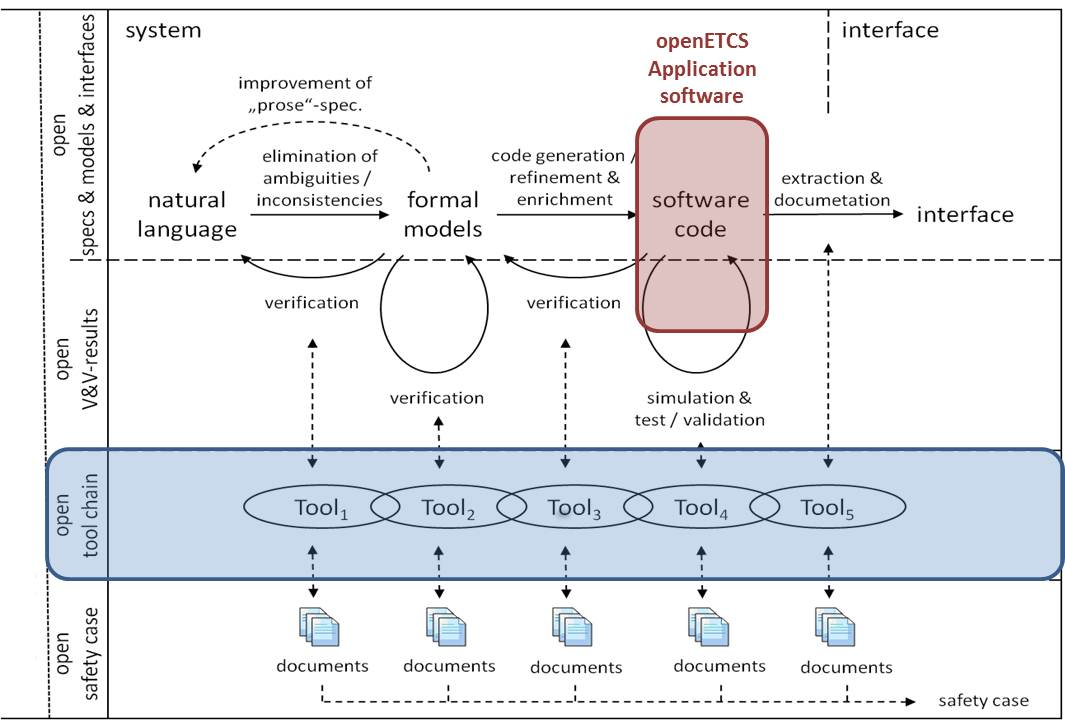
\includegraphics[width=16cm]{openETCS1}
  \caption{"open Proofs" the holistic approach}
  \label{fig:openETCS1}
\end{figure}



\section{openETCS application software}
Software code generated form formal models, see Figure \ref{fig:openETCS1} above.


\chapter{Introduction and motivation}
In all over Europe there are about 30 different, mostly not compatible signaling and train protection systems in use, see Figure \ref{fig:openETCS2}. For a unified european rail system it is very costly to maintain this diversity of signaling systems and therefore the european commission has set new rules by so called Technical Specifications for Interoperability (TSI) with the goal to implement a unified "European Train Control System (ETCS)".

\begin{figure}
\centering
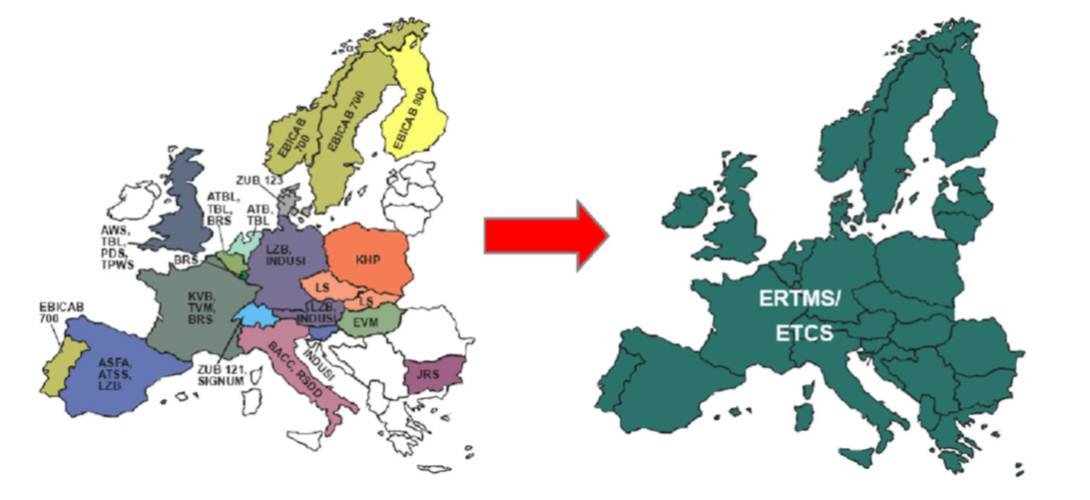
\includegraphics[width=12cm]{openETCS2}
\caption{Substitution of approximately 30 different signaling and ATP systems by just one single system: the European Train Control System (ETCS)}
\label{fig:openETCS2}
\end{figure}

ETCS is intended to replace national legacy signaling and train control systems and consists of facilities in the infrastructure and on-board units (OBU). ETCS is a so called cab-signaling system, which means that in principle all commands for the driver are shown on screens inside the driver?s cabin, making conventional track-side signals obsolete, resulting in considerable savings for the infrastructure operators. The shift of functionality and safety responsibilities from the infrastructure into the vehicle has caused an increase of complexity for the on-board equipment. In terms of technology, this is mostly done by software. While electronic hardware is getting continuously cheaper, the high complexity of the safety critical software has caused significant cost increases for development, homologation and maintenance of this technology.
Despite the fact that several major European suppliers with substantial knowledge in signal technology have worked on a common System Requirement Specification (SRS) for over a decade, the main goal of interoperability has not yet been accomplished. Up to now, not a single ETCS onboard unit has been approved to operate on all existing European ETCS lines. One of the reasons is given by the fact that a plain English specification text "prose" of some complexity cannot be so precise and free of potential divergent interpretation that the resulting software products would behave identical, see Figure \ref{fig:openETCS3}. Therefore the development of ETCS has to be considered as "work in progress", resulting in many software upgrades to be expected in the near and distant future.

\begin{figure}[h]
\centering
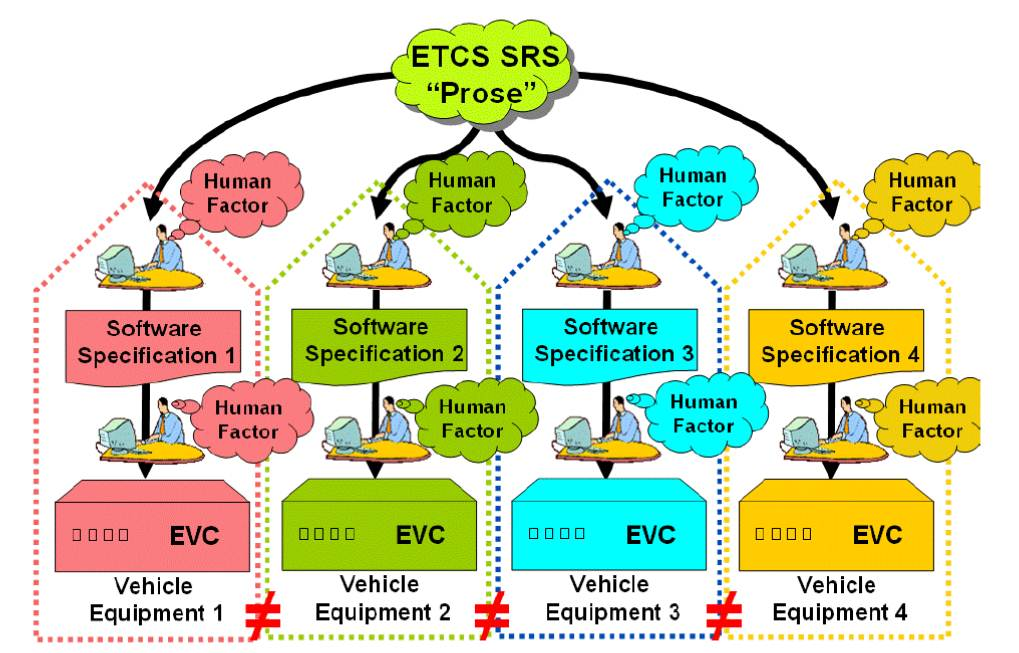
\includegraphics[width=1.0\textwidth, height=240px]{openETCS3}
\caption{Divergent interpretation of a common and mandatory public domain ETCS SRS document, due to the "human factor" by parallel working, not closely cooperating manufacturers, causing different software solutions with deviant reaction patterns, which results in interoperability deficiencies and costly subsequent retrofit works}
\label{fig:openETCS3}
\end{figure}

Almost all products on the market are based on different proprietary software designs, which results in a life-long dependency from the original manufacturers causing high life-cycle costs for vehicle owners. The key element for improving that situation seems to be a greater degree of standardization for: Hardware, software, methods and tools.
An open source approach, called "openETCS" utilizing concepts from the automotive and
aviation industry, has been suggested, not only covering the embedded application software of the ETCS onboard unit itself, but including all tools and documents in order to make the entire product life cycle as transparent as possible and make it comprehensible for third parties.
Making the proof of safety open to the public has been called "open proof" and is new to the railway sector, see Figure \ref{fig:openETCS4}.

\begin{figure}[h]
\centering
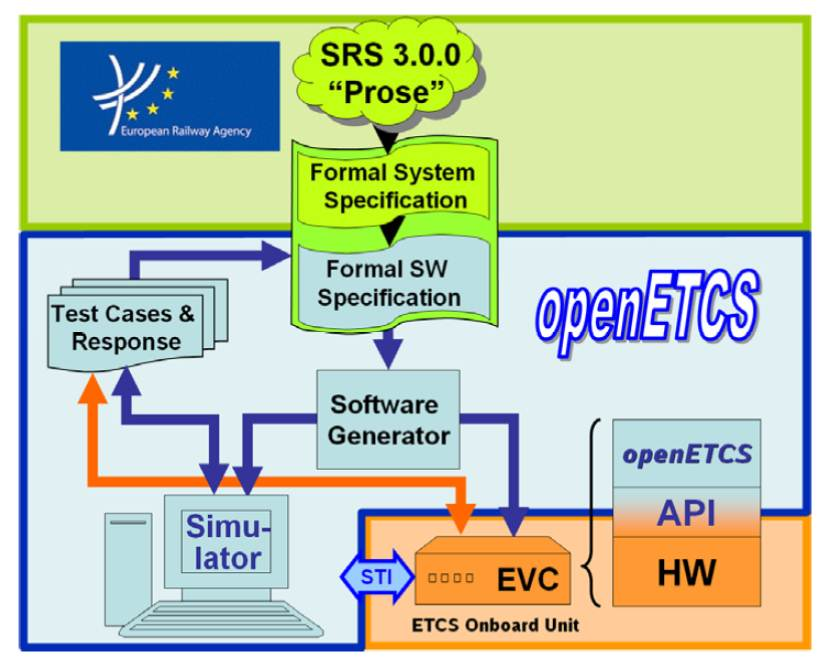
\includegraphics[width=1.0\textwidth, height=242px]{openETCS4}
\caption{openETCS approach}
\label{fig:openETCS4}
\end{figure}


\chapter{What is openETCS?}

\section{Description}
A detailed description of the project openETCS is given in the Project Outline Full Project
Proposal, see \cite{FPP13}.

\section{Main goals and deliverables}
The objective of the openETCS project is to provide a usable open source application software; including tools, documentations and the safety case for all ETCS OBU. That means, are made available as FLOSS under a "General Public License" (e.g. EUPL: European Union Public License).
\\
According to the project co-operation agreement \cite{PCA12}, The main goals and deliverables of the openETCS project are:
\begin{enumerate}
  \item Create a formal specification of the ETCS OBU functionality according to UNISIG Subset 026,
  \item Generate an executable software package from the formal specification and integrate the generated software package in the target hardware (non vital integration) for laboratory test, simulation and reference purposes,  
  \item Develop a tools chain supporting both previous bullet points including: code, test case and document generation, meeting CENELEC EN50128:2011 (T3) requirements and certifiable for SIL4 software applications for signalling equipment.
\end{enumerate}


\chapter{Purpose and creation of this report}

\section{Purpose of this report}
Due to the particularity of this project and taking into account the goals of this project, it should be clarified in advance which requirements shall be fulfilled in order to be compliant with the CENELEC standard EN 50128:2011. The work was carried out and coordinated by AEbt and the result is this report. Hence, this report elicits requirements that must be fulfilled in order to prove, that the openETCS project deliverables are fit for theirs intended purpose and responds correctly to safety issues that was derived from the System (ERTMS) Safety Requirements Specification.

\section{Creation of this report}
\label{report}
Basis for the realisation of this report were:
\begin{itemize}
  \item Articles and other technical literature
  \item Existing processes in the signalling industry
  \item CENELEC standards
\end{itemize}

This work was also carried out through interviews with experts. The experts interviewed were industrial experts, signalling experts and standardisation experts. 


\chapter{Results}

This section describes the result of the performed work.

\section{Safety requirements to be fulfilled according to EN 50128:2011}

Safety requirements according to the CENELEC standard EN 50128:2011 that shall be fulfilled by the openETCS tools chain and the openETCS application software, are recorded in annex \ref{annexA} and \ref{annexB}.


\section{Security requirements to be fulfilled}
\subsection{Introduction}
Security Requirements are not described in the standard EN 50128:2011, nevertheless due to the nature of this project and based on interviews performed with software and signalling experts, we recommend to implement the security requirements described in sections \ref{DPatterns}, \ref{CPatterns} and \ref{Backdoor}.

\subsection{Secure Design Patterns}
\label{DPatterns}
During the design of the openETCS application software, software security can be enhanced through the implementation of secure design patterns. 
Three of the most techniques used are listed below:
\begin{enumerate}
  \item Distrustful decomposition
  \item Privilege separation
  \item Clear sensitive information
\end{enumerate}

\subsubsection{Distrustful decomposition}
The intent of the Distrustful Decomposition secure design pattern is to move separate functions into mutually untrusting programs, thereby reducing:
\begin{itemize}
  \item the attack surface of the individual programs that make up the system
  \item the functionality and data exposed to an attacker if one of the mutually untrusting programs is compromised
\end{itemize}

\subsubsection{Privilege separation}
The intent of the Privilege separation is to reduce the amount of code that runs with special privilege without affecting or limiting the functionality of the program. The Privilege separation is a more specific instance of the distrustful decomposition.

\subsubsection{Clear sensitive information}
The use of this pattern ensures that sensitive information is cleared from reusable resources before the resource may be reused. It is possible that sensitive information stored in a reusable resource may be accessed by an unauthorized user or adversary if the sensitive information is not cleared before freeing the reusable resource.


\subsection{Secure coding Patterns}
\label{CPatterns}
During the implementation of the openETCS application software and tool chain, software security can be augmented by avoiding a number of common software security vulnerabilities. 
The following software security vulnerabilities shall be avoided:
\begin{enumerate}
  \item Buffer overflow
  \item Pointer shenanigans
  \item Dynamic memory allocation flaws
  \item Tainted data
\end{enumerate}

\subsubsection{Buffer overflow}
Buffer overflow can lead to more serious consequences, such as stack smashing, code injection, or even arc injection by which an attacker changes the control flow of the program by modifying the return address on stack. In arc injection, an attacker doesn't even have to inject any code, and he can jump to an arbitrary function in existing code, or bypass validity checks or assertions \cite{Kalinsky09}.

\subsubsection{Pointer shenanigans}
If an attacker can modify a data pointer, then the attacker can point to wherever he likes and write whatever he likes. If an attacker can overwrite a function pointer, the attacker is well on his way to executing his code on the processor \cite{Kalinsky09}.

\subsubsection{Dynamic memory allocation flaws}
The use of dynamic memory allocation shall be forbidden within the openETCS project. It is so easy to write defective code for dynamic memory allocation, so that attackers are eager to search out these defects \cite{Kalinsky09}.

\subsubsection{Tainted data}
Data entering an embedded system from the outside world must not be trusted. Instead, it must be "sanitized" before use \cite{Kalinsky09}.
A useful technique for data sanitization is called "white listing". It involves describing all possible valid values for a given piece of data and then writing code that only accepts those values. All unexpected values are viewed as "tainted" and are not used.


\subsection{Backdoor}
\label{Backdoor}
A backdoor can be created by each person who has access to the software source code, but it is also possible to create a backdoor without modifying the software source code, or even modifying it after compilation. This can be done by rewriting the compiler so that it recognizes code during compilation that triggers inclusion of a backdoor in the compiled output. When the compromised compiler finds such code, it compiles it as normal, but also inserts a backdoor. This attack was first outlined by Ken Thompson in his paper "Reflections on Trusting Trust" \cite{Ken84}.

A useful technique against back doors is the so called "Diverse Double-Compiling"-technic see \cite{Wheeler09}. 


\section{Recommendation for the openETCS project}

\subsection{Regarding Secure design Patterns}
The architecture and design specification of the openETCS application software shall implement the requirements described in section \ref{DPatterns}.

\subsection{Regarding Secure coding Patterns}
Since the software code of the openETCS application software will be automatically generated using tools,  tools used or developed shall avoid the software security vulnerabilities described in section \ref{CPatterns}.

\subsection{Regarding Backdoors}
Experiences from the past have shown that open source software are better positioned against backdoors than "close" software. For this reason, it is clear from the report of the European Parliament, that: "Calls on the Commission and Member States to promote software projects whose source text is made public (open-source software), as this is the only way of guaranteeing that no backdoors are built into programmes;" see \cite{EUParl}.
Since openETCS is an open source software project and according to \cite{EUParl}, no requirement regarding backdoor issues need to be considered.


\section{Requirements regarding Hardware, operating system and the bus system}
When developing software, it is mandatory to prove that the actual behavior of the software, when executed, will be consistent with the behavioral semantics of the software. 
Behavior is observable in: 
\begin{itemize}\itemsep=0pt
  \item The data domain,
  \item The time domain,
  \item The causal domain.
\end{itemize}

All of these behavioral aspects depend on both the OS and the underlying HW \cite{BraPeFe12}:
\begin{itemize}\itemsep=0pt
  \item Data transformations fail if, for example, the word length of the HW registers is inappropriate for the calculations involved.,
  \item Expected reactions miss their deadlines if, for example, the OS scheduler does not allocate appropriate amounts of CPU time to the task processing the input,
  \item Events occur in the wrong order if the OS does not provide adequate mechanisms for critical section management.
\end{itemize}

As a consequence the openETCS application software can only be validated and certified in relation to certain OS and HW capabilities.
We therefore expect that the EVC code generated from the openETCS models will reference the interface of some OS application program interface (API) providing the services necessary to ensure the proper behavior of the software to be executed. Moreover, a list of hardware capabilities to be fulfilled has to be specified. 
We propose to elaborate specification documents about OS and HW capabilities required. 

The OS specification document should specify:
\begin{itemize}\itemsep=0pt
  \item the API required by the openETCS application software (according to CENELEC standard EN 50128:2011, see \cite{EN50159}) for Software SIL 4,
  \item the scheduling capabilities (e.g., reaction to interrupts, partitioning in the time domain),
  \item the communication interfaces supported (according to CENELEC standard EN 50159:2010, see \cite{EN50159}).
\end{itemize}

Instead of specifying OS properties from scratch we suggest to adopt the well known OS specification from the ARINC 653 standard see \cite{ARINC} for which OS have been developed and are applied successfully for safety-critical tasks in the avionic domain.

The HW specification should include for example,
\begin{itemize}\itemsep=0pt
  \item The required HW architecture (according to CENELEC standard EN 50129:2003, see \cite{EN50129}),
  \item The required HW interfaces and their performance characteristics,
  \item The CPU architecture (number of cores, word length etc.),
  \item Partitioning requirements (the need of a memory management unit),
  \item Existence of real time clocks.
\end{itemize}



\chapter{Summary}
As task leader of the task D2.2 (according to \cite{FPP13}), AEbt has coordinated all the work. Basis, were the procedures listed in the section \ref{report} of this report. The result is a first set of requirements, which shall be fulfilled in order to assess the openETCS tools chain as T3 support tool and may be the openETCS application software as SIL4 software according to EN 50128:2011. \\\\Regarding the openETCS application software, it is not clear in the current version of the PCA \cite{PCA12} which software SIL it should have. However, we recommend to develop it as SIL 4 software according to EN 50128:2011, in order to provide a software or part of it as certifiable COTS software for a future use.\\\\
The question whether "open proofs" is suitable for safety railway applications, is not the matter. It is more about the software safety process applied. In fact, the applied software safety process shall fulfill the requirements of the CENELEC standard EN 50128:2011 as well as security requirements. In this report, both have been addressed.
In this document, reference was made to other standard; which however have not been addressed, see CENELEC EN 50159:2010 \cite{EN50159} and ARINC \cite{ARINC}.\\\\
Related to the standard ARINC \cite{ARINC}, an analysis shall be performed, in order to show, how it can be helpful for this project. Regarding the standard EN 50159:2010 \cite{EN50159}, we also recommend to perform an analysis, in order to find out which requirements from this standard and based on the required software SIL of the openETCS application software, shall be implemented.



%\section{Aenean imperdiet}
%\lipsum[11]


\nocite{*}

\bibliographystyle{unsrt}
\bibliography{erdc}

\appendix

\chapter{Tools development: state of the art regarding CENELEC EN 50128:2011}
\label{annexA}

\section{Introduction}
This section elicits requirements, which shall be fulfilled by the openETCS tools chain.
According to the Project Co-operation Agreement \cite{PCA12}, the openETCS tool chain shall fulfill the requirements of tools in class T3 according to EN 50128:2011. Since some of the tools of the openETCS tools chain not really need to be T3 compliant, the requirements to tools were therefore subdivided in 3 subsections:
\begin{itemize}\itemsep=0pt
  \item Subsection \ref{T1}, elicits the requirements to tool in class T1,
  \item Subsection \ref{T2}, elicits the requirements to tool in class T2 and,
  \item Subsection \ref{T3}, elicits the requirements to tool in class T3.
\end{itemize}

\subsection{How to read the tables used in this section}
Tables used in this document consist of three columns.
\begin{itemize}\itemsep=0pt
  \item Column [1] lists the requirements from the CENELEC standard EN 50128:2011. But since the standard is protected by copyright, only the requirements identification numbers are recorded there. The same requirements identification number as defined in the EN 50128:2011 is used. Each requirement text should therefore be read in the standard using the requirements identification number recorded in column [1] as reference.\\
In order to simplify the readability, some of the requirements of the standard were grouped, especially when they address the same subject; only few were left out, because they were not relevant for the tool development process.
  \item In column [2], it is described how the various requirements can be fulfilled. Everywhere where possible, recommendations were formulated.
  \item In column [3], documents that shall be created or provided are listed.
\end{itemize}


\section{Requirements for tools in class T1}
\label{T1}
Some examples of T1 tools:
\begin{itemize}\itemsep=0pt
  \item a text editor tool with no automatic code generation capabilities,
  \item a requirement support tool with no automatic code generation capabilities,
  \item a design support tool with no automatic code generation capabilities,
  \item configuration control tools.
\end{itemize}

{\footnotesize\sffamily\centering
\begin{longtable}{|p{2cm}|p{9cm}|p{3cm}|}
\caption{Requirements for tools in class T1}\\
\hline
\bfseries Requirements & \bfseries How the evidence shall be provided & \bfseries Documents to be created\\
\hline
\hline
\endhead
\hline
%\caption{Terms and definitions}
\endfoot

6.7.4.1 & Provide the evidence that tools in class T1 cooperate.
\linebreak
\linebreak
NOTE \linebreak
Tools cooperate if the outputs from one tool have suitable content and format for automatic input to a subsequent tool, thus minimizing the possibility of introducing human error in the reworking of intermediate results. & Evidence report.\\ 
\hline

\end{longtable}}



\section{Requirements for tools in class T2}
\label{T2}
Tools in class T2 includes verification and validation tools.\\
Some examples of T2 tools:
\begin{itemize}\itemsep=0pt
  \item static code analysers,
  \item test coverage monitors,
  \item theorem proving assistants,
  \item simulators and,
  \item model checkers.
\end{itemize}

{\footnotesize\sffamily\centering
\begin{longtable}{|p{2cm}|p{9cm}|p{3cm}|}
\caption{Requirements for tools in class T2}\\
\hline
\bfseries Requirements & \bfseries How the evidence shall be provided & \bfseries Documents to be created\\
\hline
\hline
\endhead
\hline
%\caption{Terms and definitions}
\endfoot

6.7.4.1 & Provide the evidence that tools in class T2 cooperate.
\linebreak
\linebreak 
NOTE \linebreak
Tools cooperate if the outputs from one tool have suitable content and format for automatic input to a subsequent tool, thus minimizing the possibility of introducing human error in the reworking of intermediate results. & Evidence report.\\ 
\hline
6.7.4.2 & Provide a justification report for the selection of tools in class T2.
\linebreak
\linebreak 
NOTE \linebreak
The justification report shall include the identification of potential failures which can be injected into the tools output and the measures to avoid or handle such failures. & Justification report.\\ 
\hline
6.7.4.3 & Provide a tool manual for each tool in class T2.
\linebreak
\linebreak
NOTE \linebreak
A manual which clearly defines the behaviour of the tool and any instructions or constraints on its use. & Tool Manual.\\ 
\hline
6.7.4.10 & Each tool in class T2 must be subject to configuration management. & See requirements 6.5.4.10 to 6.5.4.12.\\ 
\hline
6.7.4.11 & For each new version of tools in class T2 that is used, provide the evidence that the new version contains no significant new unknown faults. & Evidence report.\\ 
\hline
\end{longtable}}



\section{Requirements for tools in class T3}
\label{T3}
Some examples of T3 tools: 
\begin{itemize}\itemsep=0pt
  \item Design refinement tools,
  \item Compilers,
  \item Assemblers,
  \item linkers,
  \item binders,
  \item loaders,
  \item Code generation tools,
  \item Diagnostic tools used to maintain and monitor the software under operating conditions,
  \item Application data/algorithm tools.
\end{itemize}

{\footnotesize\sffamily\centering
\begin{longtable}{|p{2cm}|p{9cm}|p{3cm}|}
\caption{Requirements for tools in class T3}\\
\hline
\bfseries Requirements & \bfseries How the evidence shall be provided & \bfseries Documents to be created\\
\hline
\hline
\endhead
\hline
%\caption{Terms and definitions}
\endfoot

6.7.4.1 & Provide the evidence that tools in class T3 cooperate. 
\linebreak
\linebreak 
NOTE \linebreak
Tools cooperate if the outputs from one tool have suitable content and format for automatic input to a subsequent tool, thus minimizing the possibility of introducing human error in the reworking of intermediate results. & Evidence report.\\ 
\hline
6.7.4.2 & Provide a justification report for the selection of tools in class T3.
\linebreak
\linebreak 
NOTE \linebreak
The justification report shall include the identification of potential failures which can be injected into the tools output and the measures to avoid or handle such failures. & See requirement 6.7.4.4 .\\ 
\hline
6.7.4.3 & Provide a tool manual for each tool in class T3.
\linebreak
\linebreak
NOTE \linebreak
A manual which clearly defines the behaviour of the tool and any instructions or constraints on its use. & See requirement 6.7.4.4 .\\ 
\hline
6.7.4.4 and 6.7.4.5 & Provide the evidence that the output of tools in class T3 conforms to the specification of the output or failures in the output are detected.
\linebreak
\linebreak
Recommendation \linebreak
We highly recommend to develop tools in class T3 according to the CENELEC standard EN 50128:2011 for SIL 4 software.
See Section \ref{DevT3} & See Section \ref{DevT3}\\ 
\hline
\end{longtable}}


\section{Development process for tools in class T3 according to the CENELEC standard EN 50128:2011}
\label{DevT3}
\subsection{Boundary conditions for operating systems and hardware (Clause 4 according to EN 50128:2011)}
{\footnotesize\sffamily\centering
\begin{longtable}{|p{2cm}|p{9cm}|p{3cm}|}
\caption{Boundary conditions for operating systems and hardware (Clause 4 according to EN 50128:2011)}\\
\hline
\bfseries Requirements & \bfseries How the evidence shall be provided & \bfseries Documents to be created\\
\hline
\hline
\endhead
\hline
%\caption{Terms and definitions}
\endfoot

4.1 & Neither a tool nor software can be assessed, without at least specifying the capabilities and boundary conditions to be fulfilled by the operating system and hardware. 
\linebreak
\linebreak
Regarding tools in class T3, we therefore recommend to perform a risk and hazard analysis, in order to specify the boundary conditions for both: operating system and hardware.
& Boundary conditions for operating systems and hardware.\\ 
\hline
\end{longtable}}


\subsection{Management and organisation (Clause 5 according to EN 50128:2011)}
\label{clause5}
\subsubsection{Management and organisation regarding the development of tools in class T3}
The objective of this subclause is to ensure that all personnel who have responsibilities within the development of the tools are organised, empowered and capable of fulfilling their responsibilities.
{\footnotesize\sffamily\centering
\begin{longtable}{|p{2cm}|p{9cm}|p{3cm}|}
\caption{Management and organisation regarding the development tools in class T3 (Subclause 5.1 according to EN 50128:2011)}\\
\hline
\bfseries Requirements & \bfseries How the evidence shall be provided & \bfseries Documents to be created\\
\hline
\hline
\endhead
\hline
%\caption{Terms and definitions}
\endfoot

5.1.2.1 & EN ISO 9001 certification for each organisation involved in the tool development process must be provided. & EN ISO 9001 certification.\\ 
\hline
5.1.2.2, 5.1.2.3 and 5.1.2.9 to 5.1.2.14 & A quality assurance plan shall be created at the beginning of the project. 

\textbf{NOTE }
\begin{itemize}\itemsep=0pt
  \item The quality assurance plan shall be written according to subclause 6.5.
  \item The created quality assurance plan shall also implement the requirements of 5.1.2.2, 5.1.2.3, 5.1.2.9, 5.1.2.10, 5.1.2.13 and 5.1.2.14.
\end{itemize}
& Quality assurance plan\\ 
\hline
5.1.2.4 to 5.1.2.8 & Create an assessment plan for the tools. (only when required).
& Assessment Plan\\ 
\hline
\end{longtable}}

\subsubsection{Personnel Competence regarding the development of tools in class T3}
\begin{flushleft}
The objective of this subclause is to ensure that all personnel who have responsibilities for thed evelopment of tools are competent to discharge those responsibilities by demonstrating the ability to perform relevant tasks correctly, efficiently and consistently to a high quality and under varying conditions.
\end{flushleft}
{\footnotesize\sffamily\centering
\begin{longtable}{|p{2cm}|p{9cm}|p{3cm}|}
\caption{Personnel competence regarding tools in class T3 (Subclause 5.2 according to EN 50128:2011)}\\
\hline
\bfseries Requirements & \bfseries How the evidence shall be provided & \bfseries Documents to be created\\
\hline
\hline
\endhead
\hline
%\caption{Terms and definitions}
\endfoot

5.2.2.1 and 5.2.2.2 & After it has been named and recorded in the quality assurance plan who is:
\begin{itemize}\itemsep=0pt
  \item Requirements Manager,
  \item Designer,
  \item Implementer,
  \item Tester,
  \item Verifier,
  \item Integrator,
  \item Validator,
  \item Project Manager,
  \item Configuration Manager.
\end{itemize}
and what their responsibilities within the tool development process are, now it shall be proved, that these persons are competent to discharge these responsibilities.

We propose to create a kind of "openETCS people competence matrix" at the management level. 

In this document the CV of all persons involved in the project must be recorded.
Where key competencies to fulfill a role are miss-ing, trainings must be provided.
Participation in trainings shall also be recorded in this document.
& openETCS people competence matrix
\linebreak
\linebreak
NOTE\linebreak
the created people competence matrix can also be used as evidence for the openETCS application software\\ 
\hline
5.2.2.3 and 5.2.2.4 & See requirement 5.1.2.1 & ISO 9001 certificate\\ 
\hline
\end{longtable}}

\subsubsection{Lifecycle issues and documentation regarding the development of tools in class T3}
\label{SDLC}
\begin{flushleft}
The objective of this subclause is to structure the development of tools into defined phases and activities and to record all informations throughout the lifecycle.
\end{flushleft}
{\footnotesize\sffamily\centering
\begin{longtable}{|p{2cm}|p{9cm}|p{3cm}|}
\caption{Lifecycle issues and documentation regarding tools in class T3 (Subclause 5.3 according to EN 50128:2011)}\\
\hline
\bfseries Requirements & \bfseries How the evidence shall be provided & \bfseries Documents to be created\\
\hline
\hline
\endhead
\hline
%\caption{Terms and definitions}
\endfoot

5.3.2.1 and 5.3.2.3 & A lifecycle model for the development of tools shall be selected.
& The selected lifeycle model shall be described in the Quality Assurance Plan.
\linebreak
\linebreak
NOTE\linebreak
The same lifeycle model can also be used for the development of the openETCS application software\\ 
\hline
5.3.2.2 & See requirement 5.3.2.14 & See requirement 5.3.2.14\\ 
\hline
5.3.2.4 & The Quality Assurance Plan, Verification Plan, Validation Plan and Configuration Management Plan shall be drawn up at the start of the project and maintained throughout the development life cycle of the tools & See below\\ 
\hline
5.3.2.5 & Identify all the activities to be performed at each phase of the selected lifeycle model. 

For each identified activity, create a planning document at the project start.
& Planning documents\\ 
\hline
5.3.2.6 and 6.5.4.9 & A document management process shall be applied.
 
This process shall be described in a document management plan.

The created document management plan shall implement requirements of 5.3.2.6 and 6.5.4.9
& Document management plan\\ 
\hline
5.3.2.7 & 
\begin{itemize}\itemsep=0pt
  \item Create a overall notation for documents,
  \item Create a documents relationship matrix,
\end{itemize} 
& 
\begin{itemize}\itemsep=0pt
  \item Overall notation for documents,
  \item Documents relationship matrix,
\end{itemize} 


Both documents shall be referenced in the quality assurance plan\\ 
\hline
5.3.2.8 and 5.3.2.10 & Create an overall definition of terms and abbreviations to be used within the project. 

The created "overall definition of terms and abbreviations" shall implement requirements 5.3.2.8 and 5.3.2.10
& Overall definition of terms and abbreviations.
\linebreak
\linebreak
NOTE\linebreak
The created document shall be referenced in the quality assurance plan.\\ 
\hline
5.3.2.9 & Create a checklist.
 
The created checklist shall be used to verify the internal consistency of each created documents during the development of the tools.

The created checklist shall implement the requirement 5.3.2.9.
& Checklist for documents consistency check.
\linebreak
\linebreak
NOTE\linebreak
The created Checklist shall be referenced in the quality assurance plan.\\ 
\hline
5.3.2.11 & We recommend to use well-established document file formats (html, ps, pdf, rtf, odf or latex).
& The selected file formats shall be recorded in the quality assurance plan.\\ 
\hline
5.3.2.12 and 5.3.2.13 & We do not recommend to combine documents created by independent roles. 
& - \\ 
\hline
5.3.2.14 & To develop safety relevant software or tools, the use of a suitable development process model is essential. Strict finish-to-start process models such as the V-Model are suitable to develop safety-relevant software, whereas agile process models, like Scrum, are not recommended. 

Scrum does not care about dedicated roles for quality management or safety management or documentation. Therefore, application of agile methods in safety-critical systems with focus on EN 50128:2011 is still a gap which shall be analysed when using Scrum.

In fact, there is no specific process model required in the EN 50128:2011. But the standard requires certain activities and documentation with some quality according to the corresponding safety integrity level (SSIL). 

The standard EN 50128:2011 also requires the consideration of iterative development (see requirement 5.3.2.2). Therefore, an iterative process model for developing safety relevant software or tools is important.

We recommend to perform an analysis to demonstrate that scrum meets all the objectives and requirements of the EN 50128:2011 (described in clause 6, 7 and 9)
& Lifeycle cycle impact analysis report.\\ 
\hline
\end{longtable}}



\subsection{Quality assurance measures (Clause 6 according to EN 50128:2011)}
\label{clause6}
\subsubsection{Testing during the development of tools in class T3}
\begin{flushleft}
The objective of this subclause is to ascertain the behaviour or performance of the developed tool against the corresponding test specification to the extent achievable by the test coverage.
\end{flushleft}
{\footnotesize\sffamily\centering
\begin{longtable}{|p{2cm}|p{9cm}|p{3cm}|}
\caption{Testing activities during the development of tools in class T3 (Subclause 6.1 according to EN 50128:2011)}\\
\hline
\bfseries Requirements & \bfseries How the evidence shall be provided & \bfseries Documents to be created\\
\hline
\hline
\endhead
\hline
%\caption{Terms and definitions}
\endfoot

6.1.4.1 to 6.1.4.4 and 8.4.8.6 & Each created Test Specification shall implement the requirement of 6.1.4.4 and 8.4.8.6.
& Test Specifications \\ 
\hline
6.1.4.5 & Each created test report shall implement the requirement of 6.1.4.5.
& Test Reports \\ 
\hline
\end{longtable}}


\subsubsection{Verification during the development of tools in class T3}
\begin{flushleft}
The objective of this subclause is to examine and arrive at a judgment based on evidence that output items (process, documentation, software) of a specific development phase fulfill the requirements and plans with respect to completeness, correctness and consistency.
\end{flushleft}
{\footnotesize\sffamily\centering
\begin{longtable}{|p{2cm}|p{9cm}|p{3cm}|}
\caption{Verification activities during the development of tools in class T3 (Subclause 6.2 according to EN 50128:2011)}\\
\hline
\bfseries Requirements & \bfseries How the evidence shall be provided & \bfseries Documents to be created\\
\hline
\hline
\endhead
\hline
%\caption{Terms and definitions}
\endfoot

6.2.4.1 to 6.2.4.9 and 8.4.8.6 & Create a verification plan.

The created verification plan shall implement the requirement of 6.2.4.9 and 8.4.8.6.

For Verification activities, the approved combinations of techniques for software safety integrity level 4 as described in annex A, table A.5, A,6, A.7 and A.8 of EN 50128:2011 shall be selected and recorded in the created verification Plan.
& Verification Plan
\linebreak
\linebreak
NOTE\linebreak
The verification plan shall be drawn up at the start of the project and maintained throughout the tool development life cycle.\\ 
\hline
6.2.4.10 to 6.2.4.11 & Once the verification plan has been created; it shall be verified. 

The results of the verification shall be recorded in the quality assurance verification report.

The created quality assurance verification report shall implement the requirements of 6.2.4.11.
& Quality assurance verification report.\\ 
\hline
6.2.4.12 to 6.2.4.13 & Create verification reports.

Each created verification report shall implement the requirements of 6.2.4.13.
& Verification Reports.\\ 
\hline
\end{longtable}}



\subsubsection{Validation during the development of tools in class T3}
\begin{flushleft}
The objective of this subclause is to determine whether the developed tool fits the user needs, in particular with respect to safety and quality and with emphasis on the suitability of its operation in accordance to its purpose in its intended environment.
\end{flushleft}
{\footnotesize\sffamily\centering
\begin{longtable}{|p{2cm}|p{9cm}|p{3cm}|}
\caption{Validation activities during the development of tools in class T3 (Subclause 6.3 according to EN 50128:2011)}\\
\hline
\bfseries Requirements & \bfseries How the evidence shall be provided & \bfseries Documents to be created\\
\hline
\hline
\endhead
\hline
%\caption{Terms and definitions}
\endfoot

6.3.4.1 to 6.3.4.6 and 8.4.8.6 & Create a validation plan.

The created validation plan shall implement the requirements of 6.3.4.4 and 8.4.8.6.
& Validation Plan
\linebreak
\linebreak
NOTE\linebreak
The validation plan shall be drawn up at the start of the project and maintained throughout the tool development life cycle.\\ 
\hline
6.3.4.7 to 6.3.4.11 & Create a validation report.

The created validation report shall implement the requirements from 6.3.4.8 to 6.3.4.11
& Validation report.\\ 
\hline
6.3.4.13 & Once the validation plan has been created; it shall be verified.

The results of the verification shall be recorded in the validation verification report.

The created validation verification report shall implement the requirements of 6.3.4.13.
& Validation plan verification report.\\ 
\hline
6.3.4.14 & Once the validation report has been created; it shall be verified.

The results of the verification shall also be recorded in the validation verification report.

The created validation verification report shall also implement the requirements of 6.3.4.14.
& Validation verification report.\\ 
\hline
\end{longtable}}


\subsubsection{Assessment of the tools}
This section is not relevant to the tool development team. Since the assessor only assesses activities that were carried out in the clauses \ref{clause5}, \ref{clause6}, \ref{clause7}, and \ref{clause9}, the tool development team only has to implement the requirements described there correctly.


\subsubsection{Quality assurance during the development of tools in class T3}
\begin{flushleft}
The objective of this subclause is to identify, monitor and control all those activities, both technical and managerial, which are necessary to ensure that the developed tool achieves the quality required. 
\end{flushleft}
{\footnotesize\sffamily\centering
\begin{longtable}{|p{2cm}|p{9cm}|p{3cm}|}
\caption{Quality assurance activities during the development of tools in class T3 (Subclause 6.5 according to EN 50128:2011)}\\
\hline
\bfseries Requirements & \bfseries How the evidence shall be provided & \bfseries Documents to be created\\
\hline
\hline
\endhead
\hline
%\caption{Terms and definitions}
\endfoot

6.5.4.1 & See requirement 5.3.2.4 & See requirement 5.3.2.4\\ 
\hline
6.5.4.2 & See requirement 5.3.2.1 & See requirement 5.3.2.1\\ 
\hline
6.5.4.3 to 6.5.4.6 and 6.5.4.13 & Create a quality assurance plan.

The created quality assurance plan shall implement the requirements of 6.5.4.5, 6.5.4.6 and 6.5.4.13
& Quality assurance plan.
\linebreak
\linebreak
NOTE\linebreak
The quality assurance plan shall be drawn up at the start of the project and maintained throughout the tool development life cycle.\\ 
\hline
6.5.4.7 to 6.5.4.8 & Once the quality assurance plan has been created; it shall be verified.

The results of the verification shall also be recorded in the quality assurance verification report.

The created quality assurance verification report shall implement the requirements of 6.5.4.8.
& Quality assurance verification report.\\ 
\hline
6.5.4.9 & See requirement 5.3.2.6 & See requirement 5.3.2.6\\ 
\hline
6.5.4.10 to 6.5.4.12 and 9.1.4.14 & Create a configuration management plan.

The IEEE Standard for Software Configuration Management Plans (IEEE 828) can be used as guideline to create the configuration management plan.

The created configuration management plan shall also implement the requirements 6.5.4.10 to 6.5.4.12 and 9.1.4.14.
& Configuration management plan
\linebreak
\linebreak
NOTE\linebreak
The configuration management plan shall be drawn up at the start of the project and maintained throughout the tool development life cycle.\\ 
\hline
6.5.4.14 to 6.5.4.16 and 9.1.4.19 & Create a traceability matrix.

The created traceability matrix shall implement requirements from 6.5.4.14 to 6.5.4.16 and 9.1.4.19.
& Traceability matrix\\ 
\hline
6.5.4.17 & We recommend to trace all objects and documents & - \\ 
\hline
\end{longtable}}


\subsubsection{Modification and change control during the development of tools in class T3}
\begin{flushleft}
The objective of this subclause is to ensure that the tools perform as required, preserving the safety integrity and dependability when modifying the tools.
\end{flushleft}
{\footnotesize\sffamily\centering
\begin{longtable}{|p{2cm}|p{9cm}|p{3cm}|}
\caption{Modification and change control activities during the development of tools in class T3 (Subclause 6.6 according to EN 50128:2011)}\\
\hline
\bfseries Requirements & \bfseries How the evidence shall be provided & \bfseries Documents to be created\\
\hline
\hline
\endhead
\hline
%\caption{Terms and definitions}
\endfoot

6.6.4.1 to 6.6.4.2 & Applied a change management process.

The change management process shall be described in a  change management plan and shall implement the requirements from 6.6.4.1 to 6.6.4.2.
& Change Management Plan\\ 
\hline
\end{longtable}}


\subsubsection{Support tools and languages for the development of tools in class T3}
\begin{flushleft}
This subclause refers to tools that are used to develop the openETCS T3 tools.
\end{flushleft}
{\footnotesize\sffamily\centering
\begin{longtable}{|p{2cm}|p{9cm}|p{3cm}|}
\caption{Support tools and languages used for the development tools in class T3 (Subclause 6.7 according to EN 50128:2011)}\\
\hline
\bfseries Requirements & \bfseries How the evidence shall be provided & \bfseries Documents to be created\\
\hline
\hline
\endhead
\hline
%\caption{Terms and definitions}
\endfoot

6.7.4.1 & See section \ref{T1} & See section \ref{T1}\\ 
\hline
6.7.4.2 & See section \ref{T2} & See section \ref{T2}\\ 
\hline
6.7.4.3 & See section \ref{T2} & See section \ref{T2}\\  
\hline
6.7.4.4 & See requirement 6.7.4.5 & See requirement 6.7.4.5\\  
\hline
6.7.4.5 & Provide or create a tool validation.
The tool validation report shall implement the requirements of 6.7.4.5.
& Tool validation report\\  
\hline
6.7.4.6 to 6.7.4.11 & We recommend to implement requirements 6.7.4.1, 6.7.4.2, 6.7.4.3, 6.7.4.4 and 6.7.4.5.
& See requirements 6.7.4.1, 6.7.4.2, 6.7.4.3, 6.7.4.4 and 6.7.4.5\\  
\hline
\end{longtable}}


\subsection{Tools development (Clause 7 according to EN 50128:2011)}
\label{clause7}
\subsubsection{Lifecycle and documentation regarding the development of tools in class T3}
See Subsection \ref{SDLC}.


\subsubsection{Requirements for the tools in class T3 to be developed}
\begin{flushleft}
The objective of this subclause is to describe a complete set of requirements for  tools to be developed, meeting all safety requirements and provides a comprehensive set of documents for each subsequent phase and to describe the overall test specification for the tools to be developed.
\end{flushleft}
{\footnotesize\sffamily\centering
\begin{longtable}{|p{2cm}|p{9cm}|p{3cm}|}
\caption{Requirements for tools in class T3 (Subclause 7.2 according to EN 50128:2011)}\\
\hline
\bfseries Requirements & \bfseries How the evidence shall be provided & \bfseries Documents to be created\\
\hline
\hline
\endhead
\hline
%\caption{Terms and definitions}
\endfoot

7.2.4.1 to 7.2.4.14 & Specify the requirements for the tools to be developed.

The created requirements specification shall implement requirements from 7.2.4.2 to 7.2.4.15.
Requirements 7.2.4.10 and 7.2.4.11 are not relevant for tools.

Traceability proof shall be provided. (for Traceability matters see requirement 6.5.4.15)
& Requirements specification for tools.
Traceability proof\\ 
\hline
7.2.4.15 & For requirements specification, use techniques from the Table A.2 of the standard EN 50128:2011.

The techniques used, must be suitable for the software safety integrity level SIL4.
& The selected techniques shall be recorded in the Quality Assurance Plan.\\ 
\hline
7.2.4.16, 7.2.4.17 and 7.2.4.19 & Create the overall Test Specification for the tools to be developed according to the requirements of 6.1.4.4

The created overall test specification shall also implement the requirements of 7.2.4.19.
& The overall Test Specification for tools\\ 
\hline
7.2.4.18 & For the overall test specification, use techniques from the Table A.7 of the standard EN 50128:2011

The techniques used, must be suitable for the software safety integrity level SIL4
& The selected techniques shall be recorded in the Quality Assurance Plan.\\ 
\hline
7.2.4.21 and 7.2.4.22 & Once the Requirement Specification for the tools to be developed has been created; it shall be verified. 

The results of the verification shall be recorded in the tool requirements verification report.

The created tool requirements verification report shall implement the requirements of 7.2.4.22.
& Tool requirements verification report \\ 
\hline
\end{longtable}}


\subsubsection{Architecture and design for the tools in class T3 to be developed}
\begin{flushleft}
 The objective of this subclause is to develop an architecture, that achieves the requirements of the tools to be developed and to identify and evaluate the significance of the interactions of the tools with the
 \end{flushleft} hardware.
{\footnotesize\sffamily\centering
\begin{longtable}{|p{2cm}|p{9cm}|p{3cm}|}
\caption{Architecture and design for tools in class T3 (Subclause 7.3 according to EN 50128:2011)}\\
\hline
\bfseries Requirements & \bfseries How the evidence shall be provided & \bfseries Documents to be created\\
\hline
\hline
\endhead
\hline
%\caption{Terms and definitions}
\endfoot

7.3.4.1 to 7.3.4.15 & Specify the architecture for the tools to be developed.

The created architecture specification shall implement requirements from 7.3.4.1 to 7.3.4.15.
Requirement 7.3.4.4 is not relevant for tools.

Traceability proof shall be provided. (for Traceability matters see requirement 6.5.4.15)
& Architecture specification for tools.
Traceability proof\\ 
\hline
7.3.4.14 & For the architecture specification, use techniques from the Table A.3 of the standard EN 50128:2011.

The techniques used, must be suitable for the software safety integrity level SIL4
& The selected techniques shall be recorded in the Software Quality Assurance Plan.
\linebreak
\linebreak
NOTE\linebreak
The use of the technic 4 "Error Detecting Codes" of Table A.3 is mandatory.\\ 
\hline
7.3.4.16 and 7.3.4.17 & Prototyping can be used at this stage.
& Evidence that the code from a prototype and its development and documentation fulfills SIL4 according to EN 50128:2011\\ 
\hline
7.3.4.18 and 7.3.4.19 & Specify the interface for the tools to be developed.

The created Interface specification shall implement requirements from 7.3.4.18 and 7.3.4.19.
& Tool interface specification.\\ 
\hline
7.3.4.20 to 7.3.4.23, 7.3.4.28, 9.1.4.10, 9.1.4.13, 9.1.4.16 and 9.1.4.20
& Specify the design of the tools to be developed.

The created design specification shall implement requirements from 7.3.4.21 to 7.3.4.24, 7.3.4.28, 9.1.4.10, 9.1.4.13, 9.1.4.16 and 9.1.4.20.
& Tool design specification.\\ 
\hline
7.3.4.24 & For the design specification, used techniques from the Table A.4 of the standard EN 50128:2011
The techniques used, must be suitable for the software safety integrity level SIL4
& The selected techniques shall be recorded in the Quality Assurance Plan.\\ 
\hline
7.3.4.25 to 7.3.4.27 & 
Specify a coding standard.

The Coding standard specification should include:
\begin{itemize}\itemsep=0pt
  \item language justification,
  \item Scope and base standard when available, (NOTE For domain specific languages base standards may not be available.),
  \item procedure for changing the coding standard,
  \item analysis of the potential faults and recommended treatment,
  \item restrictions to avoid the faults,
  \item portability.
\end{itemize}


A Justification shall be provided that the coding standards used, satisfy the software safety integrity level SIL4.
& 
\begin{itemize}\itemsep=0pt
  \item Coding standard specification,
  \item Justification for the coding standards used.
\end{itemize}

\textbf{NOTE}\linebreak
The selected coding standards and the Justification shall be referenced in the Quality Assurance Plan.\\ 
\hline
7.3.4.29 and 7.3.4.31 & Create an integration Test Specification for the tools to be developed, according to requirement 6.1.4.4.

The created tools integration test specification shall also implement the requirements of 7.3.4.31
& Tools integration test specification.\\ 
\hline
7.3.4.32 & For the integration (software of the developed tool) and software/hardware Test Specification, used techniques from Tables A.5 and A.6 of the standard EN 50128:2011.

The techniques used, must be suitable for the software safety integrity level SIL4
& The selected techniques shall be recorded in the Quality Assurance Plan.\\ 
\hline
7.3.4.33 to 7.3.4.38 & Create a software/hardware integration test specification for the tools to be developed, according to requirement 6.1.4.4.

The created tools software/Hardware integration test specification shall also implement the requirements from 7.3.4.34 to 7.3.4.39
& The tools software/hardware integration test specification \\ 
\hline
7.3.4.39 & See requirement 7.3.4.32 & See requirement 7.3.4.32.\\ 
\hline
7.3.4.40 to 7.3.4.43 & Once the Architecture Specification-, the Design Specification, the software- and  software/hardware integration test specification for the tools to be developed have been created; they shall be verified.

The results of the verification shall be recorded in the tools software architecture and design verification report.

The created tools software architecture and design verification report shall implement requirements from 7.3.4.40 to 7.3.4.43.
& Tools software architecture and design verification report \\ 
\hline
\end{longtable}}



\subsubsection{Components design for the tools in class T3 to be developed}
\begin{flushleft}
The objective of this subclause is to develop design components that achieves the requirements of the design specification for the tools to be developed.
\end{flushleft}
{\footnotesize\sffamily\centering
\begin{longtable}{|p{2cm}|p{9cm}|p{3cm}|}
\caption{Components design for tools in class T3 (Subclause 7.4 according to EN 50128:2011)}\\
\hline
\bfseries Requirements & \bfseries How the evidence shall be provided & \bfseries Documents to be created\\
\hline
\hline
\endhead
\hline
%\caption{Terms and definitions}
\endfoot

7.4.4.1 to 7.4.4.5 & Specify the component design for the tools to be developed. 

The created component design specification shall implement requirements from 7.4.4.1 to 7.4.4.6
& Tools components design specification\\ 
\hline
7.4.4.6 & See requirement 7.3.4.24 & See requirement 7.3.4.24\\ 
\hline
7.4.4.7 to 7.4.4.9 & Create a component test specification for the tools to be developed, according to requirement 6.1.4.4.

The created tools component test Specification shall also implement requirements from 7.4.4.8 to 7.4.4.10
& Tools components test Specification\\ 
\hline
7.4.4.10 & See requirement 7.3.4.32 & See requirement 7.3.4.32.\\ 
\hline
7.4.4.11 to 7.4.4.13 & Once the components design specification and the components test specification for the tools to be developed have been created; they shall be verified.

The results of the verification shall be recorded in the tools component design verification report.

The created tools component design verification report shall implement requirements from 7.4.4.11 to 7.3.4.13.
& Tools component design verification report  \\ 
\hline
\end{longtable}}



\subsubsection{Implementation and Testing of the developed tools in class T3}
\begin{flushleft}
The objective of this subclause is to achieve a software of the developed tool, which is analysable, testable, verifiable and maintainable.
\end{flushleft}
{\footnotesize\sffamily\centering
\begin{longtable}{|p{2cm}|p{9cm}|p{3cm}|}
\caption{Implementation and tests of tools in class T3 (Subclause 7.5 according to EN 50128:2011)}\\
\hline
\bfseries Requirements & \bfseries How the evidence shall be provided & \bfseries Documents to be created\\
\hline
\hline
\endhead
\hline
%\caption{Terms and definitions}
\endfoot

7.5.4.1 to 7.5.4.4 & Create or generate the software source code of the developed tool.

The source code shall compliant with the requirements of 7.5.4.1 and 7.5.4.2.
& Software source code of the developed tool.\\ 
\hline
7.5.4.5 to 7.5.4.7 & Once the software source code of the developed tool has been created; the software source code of each component of the tools shall be tested.

The result of all software component tests of the developed tool shall be recorded in the tools software component test report.

The tools software component test report shall be written according to requirement 6.1.4.5.

The created tools software component test report shall also implement requirements from 7.5.4.6 to 7.5.4.7.
& Tools software component test report.\\ 
\hline
7.5.4.8 to 7.5.4.10 & The software source code of the developed tool shall be verified.

The results of the verification shall be recorded in the tools software component design verification report.

The created tools software component design verification report shall implement requirements from 7.4.4.11 to 7.3.4.13.
& Tools software component design verification report.\\ 
\hline
\end{longtable}}



\subsubsection{Integration of the software source code of the developed tools}
\begin{flushleft}
The objective of this subclause is to carry out the software- and software/hardware integration od the developed tools and to demonstrate that the software of the developed tools and the hardware interact correctly to perform their intended functions.
\end{flushleft}
{\footnotesize\sffamily\centering
\begin{longtable}{|p{2cm}|p{9cm}|p{3cm}|}
\caption{Integration of the software source code of the developed tools (Subclause 7.6 according to EN 50128:2011)}\\
\hline
\bfseries Requirements & \bfseries How the evidence shall be provided & \bfseries Documents to be created\\
\hline
\hline
\endhead
\hline
%\caption{Terms and definitions}
\endfoot

7.6.4.3 to 7.6.4.5 & Once each (software) component of the developed tools has been bug free tested; the integration of (software) components shall be started.

The result of the software integration test shall be recorded in the tools software integration test report.

The tools software integration test report shall be written according to requirement 6.1.4.5.

The created tools software integration test report shall also implement the requirements of 7.6.4.5
& Tools software integration test report.\\ 
\hline
7.6.4.6 & See requirement 7.3.4.32 & See requirement 7.3.4.32.\\ 
\hline
7.6.4.7 to 7.6.4.9 & Once the integration of (software) components of the developed tools has been bug free performed; the software/hardware integration shall be started.

The result of the software/hardware integration test shall be recorded in the tools software/hardware integration test report.

The tools software/hardware integration test report shall be written according to requirement 6.1.4.5.

The created tools software/hardware integration test report shall also implement the requirements of 7.6.4.9
& Tools software/hardware integration test report.\\ 
\hline
7.6.4.10 & See requirement 7.3.4.32 & See requirement 7.3.4.32.\\ 
\hline
7.6.4.11 to 7.6.4.13 & Once the tools software integration test report and the tools software/hardware integration test report have been created; they shall be verified.

The results of the verification shall be recorded in the tools software integration verification report

The created tools software integration verification report shall implement requirements from 7.6.4.11 to 7.6.4.13.
& Tools software integration verification report.\\ 
\hline
\end{longtable}}



\subsubsection{Validation of the software source code of the developed tools}
\begin{flushleft}
 The objective of this subclause is to analyse and test the integrated software source code of the developed tools and hardware to ensure compliance with the software requirements specification with particular emphasis on the functional and safety aspects according to software SIL4 and to check whether it is fit for its
 \end{flushleft} intended application.
{\footnotesize\sffamily\centering
\begin{longtable}{|p{2cm}|p{9cm}|p{3cm}|}
\caption{Validation of the software source code of the developed tools (Subclause 7.7 according to EN 50128:2011)}\\
\hline
\bfseries Requirements & \bfseries How the evidence shall be provided & \bfseries Documents to be created\\
\hline
\hline
\endhead
\hline
%\caption{Terms and definitions}
\endfoot

7.7.4.1 to 7.7.4.4 & Once the tool-software/hardware integration has been bug free performed; the overall tool-software test shall be started.

The result of the overall tool-software test shall be recorded in the overall tool-software test report.

The overall tool-software test report shall be written according to requirement 6.1.4.5.

& Overall tool-software test report.\\ 
\hline
7.7.4.6 to 7.7.4.11 & Once the overall tool-software test has been bug free performed; the tool-software validation shall be started.

The result of the tool-software validation shall be recorded in the tool validation report.

The tool validation report shall be written according to requirements 7.7.4.6 to 7.7.4.11
& Tool validation report.\\ 
\hline
7.7.4.12 & A Release Note which accompanies the delivered tool shall be created.

The release note for the tool shall be written according to the requirement 7.7.4.12
& Tool release note.\\ 
\hline
\end{longtable}}




\subsection{Development of application data or algorithms (Clause 8 according to EN 50128:2011)}
Tools for application data or algorithms are T3 tools and shall be developed according to the requirements described in clauses \ref{clause5}, \ref{clause6}, \ref{clause7} and \ref{clause9}.
\linebreak
\linebreak


\subsection{deployement and maintenance (Clause 9 according to EN 50128:2011)}
\label{clause9}
\subsubsection{Deployment of the developed tools}
\begin{flushleft}
The objective of this subclause is to ensure that the tool performs as required, preserving the required safety integrity and dependability when it is deployed in the final environment of application.
\end{flushleft}
{\footnotesize\sffamily\centering
\begin{longtable}{|p{2cm}|p{9cm}|p{3cm}|}
\caption{Deployment of the developed tools (Subclause 9.1 according to EN 50128:2011)}\\
\hline
\bfseries Requirements & \bfseries How the evidence shall be provided & \bfseries Documents to be created\\
\hline
\hline
\endhead
\hline
%\caption{Terms and definitions}
\endfoot

9.1.4.4 and 9.1.4.5 & Create a release note for the developed tools.

The created release note shall implement requirements from 9.1.4.4 to 9.1.4.5.
& Tool release note.\\ 
\hline
9.1.4.6 to 9.1.4.9 & Once the tool deployment manual has been created; it shall be verified.

The results of the verification shall be recorded in the tool deployment verification report.

The created tool deployment verification report shall implement requirements from 9.1.4.6 to 9.1.4.9.
& Tool deployment verification report.\\ 
\hline
9.1.4.10 & Provide the evidence that the executable code is coded. 
& See requirement 7.3.4.20.\\ 
\hline
9.1.4.11 and 9.1.4.12 & Create a tool tool deployment manual.

The created deployment manual shall implement the requirement of 9.1.4.12.
& Tool deployment manual.\\ 
\hline
9.1.4.13 & Incremental deployment is one of the most important properties of agile methods such as Scrum.

When using Scrum, it is highly recommended for SIL 4, that the software is designed to include facilities which assure that activation of incompatible versions of software components is excluded.

The design specification of the developed tool shall therefore implement this requirement.
& See requirement 7.3.4.20.\\ 
\hline
9.1.4.14 & The created configuration management plan shall also implement the requirements of 9.1.4.14.
& See requirement 6.5.4.10.\\ 
\hline
9.1.4.15 & Applied a rollback procedure process.
& Rollback procedure plan\\ 
\hline
9.1.4.16 & The tool-software design specification shall implement this requirement.
& See requirement 7.3.4.20.\\ 
\hline
9.1.4.17 and 9.1.4.18 & Create a tool deployment record for the developed tools.
The created deployment record shall implement the requirement 9.1.4.18.
& Tool deployment record.\\ 
\hline
9.1.4.19 & The traceability matrix shall implement this re-quirement.
& See requirement 6.5.4.14.\\ 
\hline
9.1.4.20 & The design specification of the developed tool shall implement this requirement.
& See requirement 7.3.4.20.\\ 
\hline
\end{longtable}}


\subsubsection{Maintenance of the developed tools}
\begin{flushleft}
 The objective of this subclause is to ensure that the tools performs as required, preserving the required safety integrity and dependability when making corrections, enhancements or adaptations to the tools itself.
 \end{flushleft} 
{\footnotesize\sffamily\centering
\begin{longtable}{|p{2cm}|p{9cm}|p{3cm}|}
\caption{Maintenance of the developed tools (Subclause 9.2 according to EN 50128:2011)}\\
\hline
\bfseries Requirements & \bfseries How the evidence shall be provided & \bfseries Documents to be created\\
\hline
\hline
\endhead
\hline
%\caption{Terms and definitions}
\endfoot

9.2.4.5 to 9.2.4.6 & Create a maintenance plan for the developed tools.

The created Maintenance Plan shall implement the requirement 9.2.4.6.
& Maintenance Plan for the developed tools.\\ 
\hline
9.2.4.7 to 9.2.4.10 & Create a maintenance verification report for the developed Tools.

The created maintenance verification report shall implement requirements from 9.2.4.7 to 9.2.4.10.
& Maintenance verification report.\\ 
\hline
9.2.4.12 & For maintenance activities, use techniques from the Table A.10 of the standard EN 50128:2011.

The selected techniques must be suitable for the software safety integrity level SIL4 
& The selected techniques shall be recorded in the Maintenance Plan.\\ 
\hline
9.2.4.15 and 9.2.4.16 & Create a maintenance record for the developed Tools.

The created Maintenance Record shall implement the requirements of 9.2.4.16.
& Tool Maintenance Record.\\ 
\hline
9.2.4.17 and 9.2.4.18 & Create a change record for the developed Tools.

The created change record shall implement requirements of 9.2.4.18.
& Tool change Record.\\ 
\hline
\end{longtable}}




\chapter{Software development: state of the art regarding CENELEC EN 50128:2011}
\label{annexB}
\section{Introduction}
This section elicits requirements, which shall be fulfilled by the openETCS application software (in this annex also named openETCS software).
Concerning the openETCS application software, it is not clear described in the actual version of the Project Co-operation Agreement \cite{PCA12} or Project Outline Full Project Proposal \cite{FPP13}, which software safety integrity level (SSIL) according EN 50128:2011 it should fulfill. However, to achieve a benefit of this project, we recommend to develop the openETCS application software according to EN 50128:2011 for SIL 4. 
Therefore; the subsections below address the requirements for SIL 4 Software according to EN 50128:2011.

\subsection{How to read the tables used in this section}
Tables used in this document consist of three columns.
\begin{itemize}\itemsep=0pt
  \item Column [1] lists the requirements from the CENELEC standard EN 50128:2011. But since the standard is protected by copyright, only the requirements identification numbers are recorded there. The same requirements identification number as defined in the EN 50128:2011 is used. Each requirement text should therefore be read in the standard using the requirements identification number recorded in column [1] as reference.
In order to simplify the readability, some of the requirements of the standard were grouped, especially when they address the same subject; only few were left out, because they were not relevant for the development process of the openETCS application software..
  \item In column [2], it is described how the various requirements can be fulfilled. Everywhere where possible, recommendations were formulated.
  \item In column [3], documents that shall be created or provided are listed.
\end{itemize}


\section{Software Safety Integrity Levels (Clause 4 according to EN 50128:2011)}
\label{clause42}
{\footnotesize\sffamily\centering
\begin{longtable}{|p{2cm}|p{9cm}|p{3cm}|}
\caption{Safety Integrity Levels (Clause 4 according to EN 50128:2011)}\\
\hline
\bfseries Requirements & \bfseries How the evidence shall be provided & \bfseries Documents to be created\\
\hline
\hline
\endhead
\hline
%\caption{Terms and definitions}
\endfoot

4.1 & Requirement (4.1) describes the allocation of software safety integrity levels to the openETCS appli-cation software in accordance with the CENELEC standards EN 50126 and EN 50129.
\linebreak
\linebreak
Neither a tool nor software can be assessed, without at least specifying the capabilities and boundary conditions to be fulfilled by the operating system and hardware. 
\linebreak
\linebreak
Regarding the openETCS application software, we therefore recommend to perform a risk and hazard analysis, in order to specify the boundary conditions for both: operating system and hardware.
& Boundary conditions for operating systems and hardware.\\ 
\hline
4.2 & In this document, we assume that the software safety integrity level of the openETCS application soft-ware is SIL4 according to EN 50128:2011.
& - \\ 
\hline
\end{longtable}}


\section{Management and organisation (Clause 5 according to EN 50128:2011)}
\label{clause52}
\subsection{Management and organisation for the development of the openETCS Software}
\begin{flushleft}
The objective of this subclause is to ensure that all personnel who have responsibilities within the development of the openETCS software are organised, empowered and capable of fulfilling their responsibilities.
\end{flushleft}
{\footnotesize\sffamily\centering
\begin{longtable}{|p{2cm}|p{9cm}|p{3cm}|}
\caption{Management and organisation regarding the development of the openETCS software}\\
\hline
\bfseries Requirements & \bfseries How the evidence shall be provided & \bfseries Documents to be created\\
\hline
\hline
\endhead
\hline
%\caption{Terms and definitions}
\endfoot

5.1.2.1 & EN ISO 9001 certification for each organisation involved in the development process of the openETCS software must be provided. & EN ISO 9001 certification.\\ 
\hline
5.1.2.2,5.1.2.3, 5.1.2.9 to 5.1.2.14 & A software quality assurance plan shall be created at the beginning of the project. 

It shall be written according to subclause 6.5.

The created software quality assurance plan shall also implement the requirements of 5.1.2.2, 5.1.2.3, 5.1.2.9, 5.1.2.10, 5.1.2.13 and 5.1.2.14
& software quality assurance plan.\\ 
\hline
5.1.2.4 to 5.1.2.8 & Create an assessment plan for the openETCS software. (only when required).
& openETCS software assessment plan\\ 
\hline
\end{longtable}}

\subsection{Personnel Competence}
\begin{flushleft}
The objective of this subclause is to ensure that all personnel who have responsibilities for the development of the openETCS software are competent to discharge those responsibilities by demonstrating the ability to perform relevant tasks correctly, efficiently and consistently to a high quality and under varying conditions.
\end{flushleft}
{\footnotesize\sffamily\centering
\begin{longtable}{|p{2cm}|p{9cm}|p{3cm}|}
\caption{Personnel competence regarding regarding the development of the openETCS software}\\
\hline
\bfseries Requirements & \bfseries How the evidence shall be provided & \bfseries Documents to be created\\
\hline
\hline
\endhead
\hline
%\caption{Terms and definitions}
\endfoot

5.2.2.1 and 5.2.2.2 & After it has been named and recorded in the software quality assurance plan who is:
\begin{itemize}\itemsep=0pt
  \item Requirements Manager,
  \item Designer,
  \item Implementer,
  \item Tester,
  \item Verifier,
  \item Integrator,
  \item Validator,
  \item Project Manager,
  \item Configuration Manager.
\end{itemize}
and what their responsibilities within the development process of the openETCS application software are, now it shall be proved, that these persons are competent to discharge these responsibilities.

We propose to create a kind of "openETCS people competence matrix" at the management level. In this document the CV of all persons involved in the project must be recorded.
Where key competencies to fulfill a role are missing, trainings must be provided.
Participation in trainings shall also be recorded in this document.
& openETCS people competence matrix.
\linebreak
\linebreak
NOTE\linebreak
The openETCS people competence matrix created in annex \ref{annexA}, can also be used here\\ 
\hline
5.2.2.3 and 5.2.2.4 & See requirement 5.1.2.1 & ISO 9001 certificate\\ 
\hline
\end{longtable}}

\subsection{Lifecycle issues and documentation}
\label{SDLC2}
\begin{flushleft}
The objective of this subclause is to structure the development of the openETCS software into defined phases and activities and to record all information pertinent to the software throughout the lifecycle of the software.
\end{flushleft}
{\footnotesize\sffamily\centering
\begin{longtable}{|p{2cm}|p{9cm}|p{3cm}|}
\caption{Lifecycle issues and documentation regarding the development of the openETCS software)}\\
\hline
\bfseries Requirements & \bfseries How the evidence shall be provided & \bfseries Documents to be created\\
\hline
\hline
\endhead
\hline
%\caption{Terms and definitions}
\endfoot

5.3.2.1 and 5.3.2.3 & A lifecycle model for the development of the openETCS software shall be selected.
\linebreak
\linebreak
NOTE
\begin{itemize}\itemsep=0pt
  \item The same lifeycle model used for the development of the openETCS tool chain can also be used for the development of the openETCS software.
  \item The openETCS software quality assurance plan shall also describe, how the openETCS tools chain are positioned within the chosen lifecycle model.
\end{itemize}
& The selected lifeycle model shall be described in the software quality assurance plan.\\ 
\hline
5.3.2.2 & See requirement 5.3.2.14 & See requirement 5.3.2.14\\ 
\hline
5.3.2.4 & The Quality Assurance Plan, Verification Plan, Validation Plan and Configuration Management Plan of the openETCS software shall be drawn up at the start of the project and maintained throughout the development life cycle of the openETCS software & See below\\ 
\hline
5.3.2.5 & Identify all the activities to be performed at each phase of the selected lifeycle model. 

For each identified activity, create a planning document at the project start.
& Planning documents\\ 
\hline
5.3.2.6 and 6.5.4.9 & A document management process shall be applied. 

This process shall be described in a document management plan.

The created document management plan shall implement requirements of 5.3.2.6 and 6.5.4.9
& Document management plan\\ 
\hline
5.3.2.7 & 
\begin{itemize}\itemsep=0pt
  \item Create a overall notation for documents,
  \item Create a documents relationship matrix,
\end{itemize} 
& 
\begin{itemize}\itemsep=0pt
  \item Overall notation for documents,
  \item Documents relationship matrix,
\end{itemize} 

Both shall be referenced in the software quality assurance plan of the openETCS software\\ 
\hline
5.3.2.8 and 5.3.2.10 & Create an overall definition of terms and abbreviations to be used within the project. 

The created "overall definition of terms and abbreviations" shall implement requirements 5.3.2.8 and 5.3.2.10
& Overall definition of terms and abbreviations.
\linebreak
\linebreak
NOTE\linebreak
The created document shall be referenced in the software quality assurance plan.\\ 
\hline
5.3.2.9 & Create a checklist. 

The created checklist shall be used to verify the internal consistency of each created documents during the development of the openETCS application software.

The created checklist shall implement the requirement of 5.3.2.9.
& Checklist for documents consistency check.
\linebreak
\linebreak
NOTE\linebreak
The created Checklist shall be referenced in the software quality assurance plan.\\ 
\hline
5.3.2.11 & We recommend to use well-established document file formats (html, ps, pdf, rtf, odf or latex).
& The selected file formats shall be recorded in the quality assurance plan.
\linebreak
\linebreak
NOTE\linebreak
the openETCS tools chain shall generate documents in the selected file formats\\ 
\hline
5.3.2.12 and 5.3.2.13 & We do not recommend to combine documents created by independent roles. 
& - \\ 
\hline
5.3.2.14 & To develop safety relevant software or tools, the use of a suitable development process model is essential. Strict finish-to-start process models such as the V-Model are suitable to develop safety-relevant software, whereas agile process models, like Scrum, are not recommended. 

Scrum does not care about dedicated roles for quality management or safety management or documentation. Therefore, application of agile methods in safety-critical systems with focus on EN 50128:2011 is still a gap which shall be analysed when using Scrum.

In fact, there is no specific process model required in the EN 50128:2011. But the standard requires certain activities and documentation with some quality according to the corresponding safety integrity level (SSIL). 

The standard EN 50128:2011 also requires the consideration of iterative development (see requirement 5.3.2.2). Therefore, an iterative process model for developing safety relevant software or tools is important
We recommend to perform an analysis to demon-strate that scrum meets all the objectives and requirements of the EN 50128:2011 (described in clause 6, 7 and 9)
& Lifeycle cycle impact analysis report.
\linebreak
\linebreak
NOTE\linebreak
The same report (as created in annex \ref{annexA}) can be used, when the same lifeycle model has been used.\\ 
\hline
\end{longtable}}



\section{Quality assurance measures (Clause 6 according to EN 50128:2011)}
\label{clause62}
\subsection{Testing during the development of the openETCS software}
\begin{flushleft}
The objective of this subclause is to ascertain the behaviour or performance of the developed openETCS software against the corresponding test specification to the extent achievable by the test coverage.
\end{flushleft}
{\footnotesize\sffamily\centering
\begin{longtable}{|p{2cm}|p{9cm}|p{3cm}|}
\caption{Testing activities during the development of the openETCS software (Subclause 6.1 according to EN 50128:2011)}\\
\hline
\bfseries Requirements & \bfseries How the evidence shall be provided & \bfseries Documents to be created\\
\hline
\hline
\endhead
\hline
%\caption{Terms and definitions}
\endfoot

6.1.4.1 to 6.1.4.4 & Each created test specification shall implement the requirement of 6.1.4.4.
& Test Specifications \\ 
\hline
6.1.4.5 & Each created test report shall implement the requirement of 6.1.4.5.
& Test Reports \\ 
\hline
\end{longtable}}


\subsection{Verification during the development of the openETCS software}
\begin{flushleft}
The objective of this subclause is to examine and arrive at a judgment based on evidence that output items (process, documentation, software) of a specific development phase fulfill the requirements and plans with respect to completeness, correctness and consistency.
\end{flushleft}
{\footnotesize\sffamily\centering
\begin{longtable}{|p{2cm}|p{9cm}|p{3cm}|}
\caption{Verification activities during the development of the openETCS software (Subclause 6.2 according to EN 50128:2011)}\\
\hline
\bfseries Requirements & \bfseries How the evidence shall be provided & \bfseries Documents to be created\\
\hline
\hline
\endhead
\hline
%\caption{Terms and definitions}
\endfoot

6.2.4.1 to 6.2.4.9 & Create a verification plan.

The created verification plan shall implement the requirement of 6.2.4.9.

For Verification activities, the approved combinations of techniques for software safety integrity level 4 as described in annex A, table A.5, A,6, A.7 and A.8 of EN 50128:2011 shall be selected and recorded in the created verification Plan.
& Software verification Plan
\linebreak
\linebreak
NOTE\linebreak
The Software verification Plan shall be drawn up at the start of the project and maintained throughout the openETCS software development life cycle.\\ 
\hline
6.2.4.10 to 6.2.4.11 & Once the Software verification plan has been created; it shall be verified.

The results of the verification shall be recorded in the software quality assurance verification report.

The created software quality assurance verification report shall implement the requirements of 6.2.4.11.
& Software quality assurance verification report.\\ 
\hline
6.2.4.12 to 6.2.4.13 & Create software verification reports.

Each created software verification report shall implement the requirements of 6.2.4.13.
& Software verification Reports.\\ 
\hline
\end{longtable}}



\subsection{Validation during the development of the openETCS software}
\begin{flushleft}
The objective of this subclause is to determine whether the developed openETCS software fits the user needs, in particular with respect to safety and quality and with emphasis on the suitability of its operation in accordance to its purpose in its intended environment.
\end{flushleft}
{\footnotesize\sffamily\centering
\begin{longtable}{|p{2cm}|p{9cm}|p{3cm}|}
\caption{Validation activities during the development of the openETCS software (Subclause 6.3 according to EN 50128:2011)}\\
\hline
\bfseries Requirements & \bfseries How the evidence shall be provided & \bfseries Documents to be created\\
\hline
\hline
\endhead
\hline
%\caption{Terms and definitions}
\endfoot

6.3.4.1 to 6.3.4.6 & Create a Software validation plan.

The created software validation plan shall implement the requirements of 6.3.4.4.
& Software Validation Plan
\linebreak
\linebreak
NOTE\linebreak
The software validation plan shall be drawn up at the start of the project and maintained throughout the openETCS software development life cycle.\\ 
\hline
6.3.4.7 to 6.3.4.11 & Create a software validation report.

The created software validation report shall implement the requirements from 6.3.4.8 to 6.3.4.11
& Software validation report.\\ 
\hline
6.3.4.13 & Once the software validation plan has been created; it shall be verified.

The results of the verification shall be recorded in the software validation verification report.

The created software validation verification report shall implement the requirements of 6.3.4.13.
& Software validation plan verification report.\\ 
\hline
6.3.4.14 & Once the software validation report has been created; it shall be verified.

The results of the verification shall also be recorded in the software validation verification report.

The created software validation verification report shall also implement the requirements of 6.3.4.14.
& Software Validation verification report.\\ 
\hline
\end{longtable}}


\subsection{Assessment of the openETCS software}
This section is not relevant to the openETCS software development team. Since the assessor only assesses activities that were carried out in the clauses \ref{clause42} \ref{clause52}, \ref{clause62}, \ref{clause72},  \ref{clause82} and \ref{clause92}, the openETCS software development team only has to implement the requirements described there correctly.


\subsection{Quality assurance during the development of the openETCS software}
\begin{flushleft}
The objective of this subclause is to identify, monitor and control all those activities, both technical and managerial, which are necessary to ensure that the developed the openETCS software achieves the quality required. 
\end{flushleft}
{\footnotesize\sffamily\centering
\begin{longtable}{|p{2cm}|p{9cm}|p{3cm}|}
\caption{Quality assurance activities during the development of the openETCS software (Subclause 6.5 according to EN 50128:2011)}\\
\hline
\bfseries Requirements & \bfseries How the evidence shall be provided & \bfseries Documents to be created\\
\hline
\hline
\endhead
\hline
%\caption{Terms and definitions}
\endfoot

6.5.4.1 & See requirement 5.3.2.4 & See requirement 5.3.2.4\\ 
\hline
6.5.4.2 & See requirement 5.3.2.1 & See requirement 5.3.2.1\\ 
\hline
6.5.4.3 to 6.5.4.6 and 6.5.4.13 & Create a software quality assurance plan.
The created quality assurance plan shall implement the requirements of 6.5.4.5, 6.5.4.6 and 6.5.4.13
& Software quality assurance plan.
\linebreak
\linebreak
NOTE\linebreak
The software quality assurance plan shall be drawn up at the start of the project and maintained throughout the openETCS software development life cycle.\\ 
\hline
6.5.4.7 to 6.5.4.8 & Once the software quality assurance plan has been created; it shall be verified.

The results of the verification shall also be recorded in the software quality assurance verification report.

The created software quality assurance verification report shall implement the requirements of 6.5.4.8.
& Software quality assurance verification report.\\ 
\hline
6.5.4.9 & See requirement 5.3.2.6 & See requirement 5.3.2.6\\ 
\hline
6.5.4.10 to 6.5.4.12 and 9.1.4.14 & Create a software configuration management plan.

The IEEE Standard for Software Configuration Management Plans (IEEE 828) can be used as guideline to create the software configuration management plan.
The created software configuration management plan shall also implement the requirements of 6.5.4.10, 6.5.4.11, 6.5.4.12 and 9.1.4.14.
& Software configuration management plan
\linebreak
\linebreak
NOTE\linebreak
The software configuration management plan shall be drawn up at the start of the project and maintained throughout the openETCS software development life cycle.\\ 
\hline
6.5.4.14 to 6.5.4.16 and 9.1.4.19 & Create a traceability matrix.

The created traceability matrix shall implement requirements from 6.5.4.14 to 6.5.4.16 and 9.1.4.19.
& Traceability matrix\\ 
\hline
6.5.4.17 & We recommend to trace all objects and documents & - \\ 
\hline
\end{longtable}}


\subsection{Modification and change control during the development of the openETCS software}
\begin{flushleft}
The objective of this subclause is to ensure that the openETCS software performs as required, preserving the software safety integrity and dependability when modi-fying the software.
\end{flushleft}
{\footnotesize\sffamily\centering
\begin{longtable}{|p{2cm}|p{9cm}|p{3cm}|}
\caption{Modification and change control activities during the development of the openETCS software (Subclause 6.6 according to EN 50128:2011)}\\
\hline
\bfseries Requirements & \bfseries How the evidence shall be provided & \bfseries Documents to be created\\
\hline
\hline
\endhead
\hline
%\caption{Terms and definitions}
\endfoot

6.6.4.1, 6.6.4.2 and 8.4.8.5 & Applied a change management process.

The change management process shall be described in a  software change management plan and shall implement the requirements from 6.6.4.1 to 6.6.4.2 and 8.4.8.5.
& Software change Management Plan\\ 
\hline
\end{longtable}}


\subsection{Support tools and languages for the development of the openETCS software}
\begin{flushleft}
The objective of this subclause is to provide evidence that potential failures of tools do not adversely affect the integrated toolset output in a safety related manner that is undetected by technical and/or organisational measures outside the tool.
\end{flushleft}
{\footnotesize\sffamily\centering
\begin{longtable}{|p{2cm}|p{9cm}|p{3cm}|}
\caption{Support tools and languages used for the development of the openETCS software  (Subclause 6.7 according to EN 50128:2011)}\\
\hline
\bfseries Requirements & \bfseries How the evidence shall be provided & \bfseries Documents to be created\\
\hline
\hline
\endhead
\hline
%\caption{Terms and definitions}
\endfoot

6.7.4.1 to 6.7.4.9 & Use the openETCS tools chain & openETCS tools chain documentation, see Annex \ref{annexA}\\ 
\hline
6.7.4.10 & Each tool in class T2 and T3 shall be clearly identifiable and must be subject to configuration management & See requirement 6.5.4.10 to 6.5.4.12\\ 
\hline
6.7.4.11 & For each new version of tools in class T2 and T3 that is used, provide the evidence that the new version contains no significant new unknown faults. & Evidence report\\  
\hline
\end{longtable}}



\section{Generic openETCS Software development (Clause 7 according to EN 50128:2011)}
\label{clause72}
\subsection{Lifecycle and documentation regarding the development of the openETCS software}
See Subsection \ref{clause52}.


\subsection{openETCS Software requirements}
\begin{flushleft}
The objective of this subclause is to describe a complete set of requirements for the openETCS software meeting all safety requirements and provides a comprehensive set of documents for each subsequent phase and to describe the overall test specification of the openETCS software.
\end{flushleft}
{\footnotesize\sffamily\centering
\begin{longtable}{|p{2cm}|p{9cm}|p{3cm}|}
\caption{Requirements for the openETCS (Subclause 7.2 according to EN 50128:2011)}\\
\hline
\bfseries Requirements & \bfseries How the evidence shall be provided & \bfseries Documents to be created\\
\hline
\hline
\endhead
\hline
%\caption{Terms and definitions}
\endfoot

7.2.4.1 to 7.2.4.14 and 8.4.8.2 & Specify the requirements of the openETCS software.

The created software requirements specification shall implement requirements from 7.2.4.2 to 7.2.4.15 and 8.4.8.2.
\linebreak
\linebreak
Traceability proof shall be provided. (for Traceability matters see requirement 6.5.4.15)
& Requirements specification for tools.
Traceability proof\\ 
\hline
7.2.4.15 & For requirements specification, use techniques from the Table A.2 of the standard EN 50128:2011.

The techniques used, must be suitable for the software safety integrity level SIL4.
& The selected techniques shall be recorded in the software quality assurance plan.\\ 
\hline
7.2.4.16, 7.2.4.17 and 7.2.4.19 & Create the overall Test Specification for the openETCS software according to the requirements of 6.1.4.4.

The created overall test specification shall also implement the requirements of 7.2.4.19.
& Overall Test Specification for the openETCS software \\ 
\hline
7.2.4.18 & For the overall test specification, use techniques from the Table A.7 of the standard EN 50128:2011.

The techniques used, must be suitable for the software safety integrity level SIL4
& The selected techniques shall be recorded in the software quality assurance plan.\\ 
\hline
7.2.4.21 and 7.2.4.22 & Once the Requirement Specification for the openETCS software has been created; it shall be verified. 

The results of the verification shall be recorded in the software requirements verification report.

The created software requirements verification report shall implement the requirements of 7.2.4.22.
& software requirements verification report \\ 
\hline
\end{longtable}}


\subsubsection{openETCS Software Architecture and Design}
\begin{flushleft}
The objective of this subclause is to develop an architecture of the openETCS software that achieves the requirements of the software and to identify and evaluate the significance of the interactions of the openETCS software with the hardware.
\end{flushleft}
{\footnotesize\sffamily\centering
\begin{longtable}{|p{2cm}|p{9cm}|p{3cm}|}
\caption{Architecture and design for the openETCS software (Subclause 7.3 according to EN 50128:2011)}\\
\hline
\bfseries Requirements & \bfseries How the evidence shall be provided & \bfseries Documents to be created\\
\hline
\hline
\endhead
\hline
%\caption{Terms and definitions}
\endfoot

7.3.4.1 to 7.3.4.15 & Specify the architecture of the openETCS software.

The created architecture specification shall imple-ment requirements from 7.3.4.2 to 7.3.4.15.
\linebreak
\linebreak
Traceability proof shall be provided. (for Traceability matters see requirement 6.5.4.15)
& Architecture specification for the openETCS software.
Traceability proof\\ 
\hline
7.3.4.14 & For the architecture specification, use techniques from the Table A.3 of the standard EN 50128:2011.

The techniques used, must be suitable for the software safety integrity level SIL4
& The selected techniques shall be recorded in the software quality assurance plan.
\linebreak
\linebreak
NOTE\linebreak
The use of the technic 4 "Error Detecting Codes" of Table A.3 is mandatory.\\ 
\hline
7.3.4.16 and 7.3.4.17 & Prototyping can be used at this stage.
& Evidence that the code from a prototype and its development and documentation fulfills SIL4 according to EN 50128:2011\\ 
\hline
7.3.4.18, 7.3.4.19 and 8.4.8.3 & Specify the interface of the openETCS software.
 
The created software interface specification shall implement the requirements of 7.3.4.18, 7.3.4.19 and 8.4.8.3.
& Software interface specification for the openETCS software.\\ 
\hline
7.3.4.20 to 7.3.4.23, 7.3.4.28, 8.4.8.7, 9.1.4.10, 9.1.4.13, 9.1.4.16 and 9.1.4.20
& Specify the design of the openETCS software.

The created design specification shall implement requirements from 7.3.4.20 to 7.3.4.24, 7.3.4.28, 8.4.8.7, 9.1.4.10, 9.1.4.13, 9.1.4.16 and 9.1.4.20.
& Software design specification for the openETCS software.\\ 
\hline
7.3.4.24 & For the design specification, used techniques from the Table A.4 of the standard EN 50128:2011.

The techniques used, must be suitable for the software safety integrity level SIL4
& The selected techniques shall be recorded in the software quality assurance plan.\\ 
\hline
7.3.4.25 to 7.3.4.27 & 
Specify a coding standard.

The Coding standard specification should include:
\begin{itemize}\itemsep=0pt
  \item language justification,
  \item Scope and base standard when available, (NOTE For domain specific languages base standards may not be available.),
  \item procedure for changing the coding standard,
  \item analysis of the potential faults and recommended treatment,
  \item restrictions to avoid the faults,
  \item portability.
\end{itemize}

A Justification shall be provided that the coding standards used, satisfy the software safety integrity level SIL4.
& 
\begin{itemize}\itemsep=0pt
  \item Coding standard specification,
  \item Justification for the coding standards used.
\end{itemize}

The selected coding standards and the Justification shall be referenced in the software quality assurance plan.\\ 
\hline
7.3.4.29 and 7.3.4.31 & Create an integration Test Specification for the openETCS software, according to requirement 6.1.4.4.

The created openETCS software integration test specification shall also implement the requirements of 7.3.4.31
& openETCS software integration test specification.\\ 
\hline
7.3.4.32 & For the integration and software/hardware Test Specification, used techniques from Tables A.5 and A.6 of the standard EN 50128:2011.

The techniques used, must be suitable for the software safety integrity level SIL4
& The selected techniques shall be recorded in the software quality assurance plan.\\ 
\hline
7.3.4.33 to 7.3.4.38 & Create a software/hardware integration test specification for the openETCS software, according to requirement 6.1.4.4.

The created openETCS software/Hardware integration test specification shall also implement the requirements from 7.3.4.34 to 7.3.4.39
& openETCS software/hardware integration test specification\\ 
\hline
7.3.4.39 & See requirement 7.3.4.32 & See requirement 7.3.4.32.\\ 
\hline
7.3.4.40 to 7.3.4.43 & Once the Architecture Specification-, the Design Specification, the software- and  software/hardware integration test specification for the openETCS software have been created; they shall be verified.

The results of the verification shall be recorded in the software architecture and design verification report.

The created openETCS software architecture and design verification report shall implement requirements from 7.3.4.40 to 7.3.4.43.
& openETCS software architecture and design verification report \\ 
\hline
\end{longtable}}



\subsection{openETCS software Component design}
\begin{flushleft}
The objective of this subclause is to develop a software design component that achieves the requirements of the openETCS software design specification to the extent required by the software safety integrity level.
\end{flushleft}
{\footnotesize\sffamily\centering
\begin{longtable}{|p{2cm}|p{9cm}|p{3cm}|}
\caption{Components design for the openETCS software (Subclause 7.4 according to EN 50128:2011)}\\
\hline
\bfseries Requirements & \bfseries How the evidence shall be provided & \bfseries Documents to be created\\
\hline
\hline
\endhead
\hline
%\caption{Terms and definitions}
\endfoot

7.4.4.1 to 7.4.4.5 & Specify the component design for the the openETCS software.
 
The created openETCS software component design specification shall implement requirements from 7.4.4.1 to 7.4.4.6
& openETCS software components design specification\\ 
\hline
7.4.4.6 & See requirement 7.3.4.24 & See requirement 7.3.4.24\\ 
\hline
7.4.4.7 to 7.4.4.9 & Create a component test specification for the openETCS software, according to requirement 6.1.4.4.

The created openETCS software component test Specification shall also implement requirements from 7.4.4.8 to 7.4.4.10
& openETCS software components test Specification\\ 
\hline
7.4.4.10 & See requirement 7.3.4.32 & See requirement 7.3.4.32.\\ 
\hline
7.4.4.11 to 7.4.4.13 & Once the components design specification and the components test specification for the openETCS software have been created; they shall be verified.

The results of the verification shall be recorded in the openETCS software component design verification report.

The created openETCS software component design verification report shall implement requirements from 7.4.4.11 to 7.3.4.13.
& openETCS software component design verification report  \\ 
\hline
\end{longtable}}



\subsection{openETCS Software implementation and testing}
\begin{flushleft}
The objective of this subclause is to achieve software which is analysable, testable, verifiable and maintainable.
\end{flushleft}
{\footnotesize\sffamily\centering
\begin{longtable}{|p{2cm}|p{9cm}|p{3cm}|}
\caption{Implementation and tests of the openETCS software (Subclause 7.5 according to EN 50128:2011)}\\
\hline
\bfseries Requirements & \bfseries How the evidence shall be provided & \bfseries Documents to be created\\
\hline
\hline
\endhead
\hline
%\caption{Terms and definitions}
\endfoot

7.5.4.1 to 7.5.4.4 & Create or generate the openETCS software source code.

The source code shall be compliant with the requirements of 7.5.4.1 and 7.5.4.2.
& openETCS Software source code.\\ 
\hline
7.5.4.5 to 7.5.4.7 & Once the openETCS software source code has been created; each openETCS software component shall be tested.

The result of all openETCS software component tests shall be recorded in the openETCS software component test report.

The openETCS software component test report shall be written according to requirement 6.1.4.5.

The created openETCS software component test report shall also implement requirements from 7.5.4.6 to 7.5.4.7.
& openETCS software component test report.\\ 
\hline
7.5.4.8 to 7.5.4.10 & The openETCS software source code shall be verified.

The results of the verification shall be recorded in the openETCS software component design verification report.

The created openETCS software component design verification report shall implement requirements from 7.4.4.11 to 7.3.4.13.
& openETCS software component design verification report.\\ 
\hline
\end{longtable}}



\subsection{openETCS Software Integration}
\begin{flushleft}
The objective of the openETCS software integration is to carry out openETCS software and software/hardware integration and emonstrate that the openETCS software and the hardware interact correctly to perform their intended functions.
\end{flushleft}
{\footnotesize\sffamily\centering
\begin{longtable}{|p{2cm}|p{9cm}|p{3cm}|}
\caption{Integration of the openETCS software source code (Subclause 7.6 according to EN 50128:2011)}\\
\hline
\bfseries Requirements & \bfseries How the evidence shall be provided & \bfseries Documents to be created\\
\hline
\hline
\endhead
\hline
%\caption{Terms and definitions}
\endfoot

7.6.4.3 to 7.6.4.5 & Once each openETCS software component has been bug free tested; the integration of openETCS software components shall be started.

The result of the openETCS software integration test shall be recorded in the openETCS software integration test report.

The openETCS software integration test report shall be written according to requirement 6.1.4.5.

The created openETCS software integration test report shall also implement the requirements of 7.6.4.5
& openETCS software integration test report.\\ 
\hline
7.6.4.6 & See requirement 7.3.4.32 & See requirement 7.3.4.32.\\ 
\hline
7.6.4.7 to 7.6.4.9 & Once the integration of openETCS software components has been bug free performed; the openETCS software/hardware integration shall be started.

The result of the openETCS software/hardware integration test shall be recorded in the openETCS software/hardware integration test report.

The openETCS software/hardware integration test report shall be written according to requirement 6.1.4.5.

The created openETCS software/hardware integration test report shall also implement the requirements of 7.6.4.9
& openETCS software/hardware integration test report.\\ 
\hline
7.6.4.10 & See requirement 7.3.4.32 & See requirement 7.3.4.32.\\ 
\hline
7.6.4.11 to 7.6.4.13 & Once the openTCS software integration test report and software/hardware integration test report have been created; they shall be verified.

The results of the verification shall be recorded in the openETCS software integration verification report.

The created openETCS software integration verification report shall implement requirements from 7.6.4.11 to 7.6.4.13.
& openETCS software integration verification report.\\ 
\hline
\end{longtable}}



\subsection{openETCS Software Validation}
\label{ValSW}
\begin{flushleft}
The objective of the software validation is to analyse and test the integrated openETCS software and hardware to ensure compliance with the software requirements specification with particular emphasis on the functional and safety aspects according to software SIL4 and to check whether it is fit for its intended application.
\end{flushleft}
{\footnotesize\sffamily\centering
\begin{longtable}{|p{2cm}|p{9cm}|p{3cm}|}
\caption{Validation of the openETCS software source code  (Subclause 7.7 according to EN 50128:2011)}\\
\hline
\bfseries Requirements & \bfseries How the evidence shall be provided & \bfseries Documents to be created\\
\hline
\hline
\endhead
\hline
%\caption{Terms and definitions}
\endfoot

7.7.4.1 to 7.7.4.4 & Once the openETCS software/hardware integration has been bug free performed; the overall openETCS software test shall be started.

The result of the overall openETCS software test shall be recorded in the overall openETCS soft-ware test report.

The openETCS software test report. shall be writ-ten according to requirement 6.1.4.5.
& Overall openETCS software test report.\\ 
\hline
7.7.4.6 to 7.7.4.11 & Once the overall openETCS software test has been bug free performed; the openETCS software validation shall be started.

The result of the openETCS software validation shall be recorded in the openETCS software validation report.

The openETCS software validation report shall be written according to requirements 7.7.4.6 to 7.7.4.11
& openETCS software validation report.\\ 
\hline
7.7.4.12 and 8.4.8.8 & A Release Note which accompanies the delivered openETCS software shall be created.

The release note for the openETCS software shall be written according to the requirements of 7.7.4.12 and 8.4.8.8.
& openETCS software release note.\\ 
\hline
\end{longtable}}




\section{Development of application data or algorithms (Clause 8 according to EN 50128:2011)}
\label{clause82}

\subsection{Application Data Development Process}
{\footnotesize\sffamily\centering
\begin{longtable}{|p{2cm}|p{9cm}|p{3cm}|}
\caption{Development process of application data of the generic openETCS software (Subclause 8.4.1 according to EN 50128:2011)}\\
\hline
\bfseries Requirements & \bfseries How the evidence shall be provided & \bfseries Documents to be created\\
\hline
\hline
\endhead
\hline
%\caption{Terms and definitions}
\endfoot

8.4.1.2 to 8.4.1.11 and 8.4.4.1 & Created an application preparation plan for the application data of the openETCS application software.

The created application preparation plan shall implement requirements from 8.4.1.2 to 8.4.1.11 and 8.4.4.1
& openETCS Application data preparation plan.\\ 
\hline
8.4.1.12 to 8.4.1.13 & Once the openETCS application preparation plan has been created; it shall be veri-fied.

The results of the verification shall be recorded in the openETCS application data verification report.

The created application data verification report shall implement the requirement of 8.4.1.13.
& openETCS application data verification report.\\ 
\hline
\end{longtable}}


\subsection{Application Data Requirements Specification}
{\footnotesize\sffamily\centering
\begin{longtable}{|p{2cm}|p{9cm}|p{3cm}|}
\caption{Requirements Specification of application data of the generic openETCS software (Subclause 8.4.2 according to EN 50128:2011)}\\
\hline
\bfseries Requirements & \bfseries How the evidence shall be provided & \bfseries Documents to be created\\
\hline
\hline
\endhead
\hline
%\caption{Terms and definitions}
\endfoot

8.4.2.1 to 8.4.2.3 & Specify the requirements of the  application data of the openETCS software.

The created openETCS application data requirements specification shall implement requirements from 8.4.2.1 to 8.4.2.3.
& openETCS application data requirements specification.\\ 
\hline
8.4.2.4 and 8.4.2.5 & Once the openETCS application data requirements specification has been created; it shall be verified.

The results of the verification shall be recorded in the openETCS application data verification report.

The created openETCS application data verification report shall im-plement the requirements of 8.4.2.5.
& openETCS application data verification report.\\ 
\hline
\end{longtable}}


\subsection{Application Data Architecture and Design}
{\footnotesize\sffamily\centering
\begin{longtable}{|p{2cm}|p{9cm}|p{3cm}|}
\caption{Architecture and design of application data of the generic openETCS software (Subclause 8.4.3 according to EN 50128:2011)}\\
\hline
\bfseries Requirements & \bfseries How the evidence shall be provided & \bfseries Documents to be created\\
\hline
\hline
\endhead
\hline
%\caption{Terms and definitions}
\endfoot

8.4.3.1  & Specify the architecture and Design of the application data of the openETCS application software.
& openETCS application data architecture and design specification.\\ 
\hline
\end{longtable}}


\subsection{Application Data Production}
{\footnotesize\sffamily\centering
\begin{longtable}{|p{2cm}|p{9cm}|p{3cm}|}
\caption{Production of application data of the generic openETCS software (Subclause 8.4.4 according to EN 50128:2011)}\\
\hline
\bfseries Requirements & \bfseries How the evidence shall be provided & \bfseries Documents to be created\\
\hline
\hline
\endhead
\hline
%\caption{Terms and definitions}
\endfoot

8.4.4.3 & Create an application test report.

The test report can be written according to requirement 6.1.4.5.
& openETCS application data test report.\\ 
\hline
8.4.4.4 & Create an application Preparation Verification Report.

The openETCS application preparation verification report shall be created according to the requirement of 8.4.4.4.
& openETCS application data preparation verification report.\\ 
\hline
8.4.4.5 and 8.4.4.6 & Create an application Test Specification.

The openETCS Application Test Specification shall be created according to the requirement of 8.4.4.6.
& openETCS Application data Test Specification.\\ 
\hline
8.4.4.7 and 8.4.4.8 & Create an application Data Verification Report.

The openETCS Application Data Verification Report shall be created according to the requirement of 8.4.4.8.
& openETCS Application Data Verification Report.\\ 
\hline
\end{longtable}}


\subsection{Application Data Integration and Testing Acceptance}
{\footnotesize\sffamily\centering
\begin{longtable}{|p{2cm}|p{9cm}|p{3cm}|}
\caption{Integration and Tests of application data of the generic openETCS software (Subclause 8.4.5 according to EN 50128:2011)}\\
\hline
\bfseries Requirements & \bfseries How the evidence shall be provided & \bfseries Documents to be created\\
\hline
\hline
\endhead
\hline
%\caption{Terms and definitions}
\endfoot

8.4.5.1 and 8.4.5.2 & Created a test specification for the application data of the openETCS application software.

The created application test specification shall implement the requirement of 8.4.5.2
& openETCS application data test specification.\\ 
\hline
8.4.5.3 and 8.4.5.4 & Once the openETCS application data test specification has been created; it shall be verified.

The results of the verification shall be recorded in the openETCS application data verification report.

The created openETCS application data verification report shall implement the requirements of 8.4.5.4.
& openETCS application data verification report
\linebreak
\linebreak
NOTE\linebreak
The test report can be written according to requirement 6.2.4.12.\\ 
\hline
\end{longtable}}


\subsection{Application Data validation}
The validation of the application data of the openETCS software shall be carried outaccording to subclause \ref{ValSW}.



\subsection{Application Data preparation procedures and tools}
{\footnotesize\sffamily\centering
\begin{longtable}{|p{2cm}|p{9cm}|p{3cm}|}
\caption{preparation procedures and tools of application data of the generic openETCS software (Subclause 8.4.7 according to EN 50128:2011)}\\
\hline
\bfseries Requirements & \bfseries How the evidence shall be provided & \bfseries Documents to be created\\
\hline
\hline
\endhead
\hline
%\caption{Terms and definitions}
\endfoot

8.4.7.1 and 8.4.7.2 & Tools for the development of application data respectively to specify the generic openETCS application software, shall fulfill the requirements for tools in class T3 according to EN 50128:2011
& See Annex \ref{annexA}.
NOTE
Use the openETCS tool chain.\\ 
\hline
8.4.7.3 and 8.4.7.4 & See subclause \ref{clause92}. & See subclause \ref{clause92}.\\ 
\hline
8.4.7.5 & A configuration management plan for application data shall be created.
\linebreak
\linebreak
NOTE\linebreak
The configuration management plan for application data shall be separated from the configuration management of the openETCS application software
& openETCS Configuration management plan for applica-tion data.\\ 
\hline
\end{longtable}}


\subsection{Application Data: Development of Generic Software}
{\footnotesize\sffamily\centering
\begin{longtable}{|p{2cm}|p{9cm}|p{3cm}|}
\caption{Additional requirements for the development of the generic openETCS software (Subclause 8.4.8 according to EN 50128:2011)}\\
\hline
\bfseries Requirements & \bfseries How the evidence shall be provided & \bfseries Documents to be created\\
\hline
\hline
\endhead
\hline
%\caption{Terms and definitions}
\endfoot

8.4.8.2 & Requirement 8.4.8.2 shall be implemented in the openETCS software requirements specification 
& See requirement 7.2.4.1.\\ 
\hline
8.4.8.3 & Requirement 8.4.8.3 shall be implemented in the openETCS software interface specification. & See requirement 7.3.4.18.\\ 
\hline
8.4.8.4 & The openETCS software must be independent from the application data/algorithms. & This requirement shall be recorded in the software quality assurance plan of the openETCS software.\\ 
\hline
8.4.8.5 & Requirement 8.4.8.5 shall be implemented in the Change Management Process of the openETCS software. & See requirement 6.6.4.1.\\ 
\hline
8.4.8.6 & Requirement 8.4.8.6 shall be implemented in the software test plan, software verification plan and software validation plan of the openETCS software. & See requirements 6.1.4.1, 6.2.4.1 and  6.3.4.1.\\ 
\hline
8.4.8.7 & Requirement 8.4.8.7 shall be implemented in the software design specification of the openETCS software. & See requirement 7.3.4.20.\\ 
\hline
8.4.8.8 & Requirement 8.4.8.8 shall be implemented in the Release Note of the openETCS software. & See requirement 7.7.4.12.\\ 
\hline
\end{longtable}}





\section{deployement and maintenance (Clause 9 according to EN 50128:2011)}
\label{clause92}
\subsection{openETCS Software deployment}
\begin{flushleft}
The objective of this subclause is to ensure that the openETCS software performs as required, preserving the required software safety integrity level and dependability when it is deployed in the final environment of application (non vital OBU).
\end{flushleft}
{\footnotesize\sffamily\centering
\begin{longtable}{|p{2cm}|p{9cm}|p{3cm}|}
\caption{Deployment of the openETCS Software (Subclause 9.1 according to EN 50128:2011)}\\
\hline
\bfseries Requirements & \bfseries How the evidence shall be provided & \bfseries Documents to be created\\
\hline
\hline
\endhead
\hline
%\caption{Terms and definitions}
\endfoot

9.1.4.4 and 9.1.4.5 & Create a release note for the openETCS software.

The created release note shall implement require-ments from 9.1.4.4 to 9.1.4.5.
& openETCS release note.\\ 
\hline
9.1.4.6 to 9.1.4.9 & Once the openETCS deployment manual has been created; it shall be verified.

The results of the verification shall be recorded in the openETCS deployment verification report.

The created openETCS deployment verification report shall implement requirements from 9.1.4.6 to 9.1.4.9.
& openETCS deployment verification report.\\ 
\hline
9.1.4.10 & Provide the evidence that the executable code is coded. 
& See requirement 7.3.4.20.\\ 
\hline
9.1.4.11 and 9.1.4.12 & Create a tool deployment manual.

The created openETCS deployment manual shall implement the requirement of 9.1.4.12.& openETCS deployment manual.\\ 
\hline
9.1.4.13 & Incremental deployment is one of the most important properties of agile methods such as Scrum.

When using Scrum, it is highly recommended for SIL 4, that the software is designed to include facilities which assure that activation of incompatible versions of software components is excluded.

The software design specification of the openETCS software shall therefore implement this requirement.
& See requirement 7.3.4.20.\\ 
\hline
9.1.4.14 & The created configuration management plan shall also implement the requirements of 9.1.4.14.
& See requirement 6.5.4.10.\\ 
\hline
9.1.4.15 & Applied a rollback procedure process.
& Rollback procedure plan.\\ 
\hline
9.1.4.16 & The software design specification of the openETCS application software shall implement this requirement.
& See requirement 7.3.4.20.\\ 
\hline
9.1.4.17 and 9.1.4.18 & Create an openETCS software deployment record for the openETCS software.

The created openETCS software deployment rec-ord shall implement the requirement 9.1.4.18.
& openETCS software deployment record.\\ 
\hline
9.1.4.19 & The traceability matrix shall implement this requirement.
& See requirement 6.5.4.14.\\ 
\hline
9.1.4.20 & The software design specification of the openETCS application software shall implement this requirement.
& See requirement 7.3.4.20.\\ 
\hline
\end{longtable}}


\subsection{openETCS Software maintenance}
\begin{flushleft}
The objective of this subclause is to ensure that the openETCS software performs as required, pre-serving the required software safety integrity level and dependability when making corrections, en-hancements or adaptations to the openETCS software itself. 
\end{flushleft}
{\footnotesize\sffamily\centering
\begin{longtable}{|p{2cm}|p{9cm}|p{3cm}|}
\caption{Maintenance of the openETCS Software (Subclause 9.2 according to EN 50128:2011)}\\
\hline
\bfseries Requirements & \bfseries How the evidence shall be provided & \bfseries Documents to be created\\
\hline
\hline
\endhead
\hline
%\caption{Terms and definitions}
\endfoot

9.2.4.5 to 9.2.4.6 & Create a software maintenance plan for the openETCS software.

The created openETCS software maintenance plan shall implement the requirement 9.2.4.6.
& openETCS software maintenance plan.\\ 
\hline
9.2.4.7 to 9.2.4.10 & Create a software maintenance verification report for the openETCS software.

The created openETCS software maintenance verification report shall implement requirements from 9.2.4.8 to 9.2.4.10.
& openETCS software maintenance verification report.\\ 
\hline
9.2.4.12 & For maintenance activities, use techniques from the Table A.10 of the standard EN 50128:2011.

The selected techniques must be suitable for the software safety integrity level SIL4 
& The selected techniques shall be recorded in the Maintenance Plan.\\ 
\hline
9.2.4.15 and 9.2.4.16 & Create a software maintenance record for the openETCS software.

The created openETCS software maintenance record shall implement the requirement 9.2.4.16.
& openETCS software maintenance record.\\ 
\hline
9.2.4.17 and 9.2.4.18 & Create a software change record for the openETCS software.

The created openETCS software maintenance record shall implement requirements from 9.2.4.18.
& openETCS software maintenance record.\\ 
\hline
\end{longtable}}



\begin{thebibliography}{99}

 \bibitem{BraPeFe12}
  Cecile Braunstein, Jan Peleska, Johannes Feuser\\
  \emph{Position paper on openETCS development work flow and associated tools}\\
  University of Bremen,
  October 2012.

\bibitem{EN50126}
  European Committee for Electrotechnical Standardization\\EN 50126\\
  \emph{Railway applications - The specification and demonstration of Reliability, Availability, Maintainability and Safety (RAMS)- Part 1: Basic requirements and generic process}\\
  1999.

\bibitem{EN50128}
  European Committee for Electrotechnical Standardization\\EN 50128\\
  \emph{Railway applications - Communication, signalling and processing systems - Software for railway control and protection systems}\\
  2011.

\bibitem{EN50129}
  European Committee for Electrotechnical Standardization\\EN 50129\\
  \emph{Railway applications - Communication, signalling and processing systems- Safety related electronic systems for signalling}\\
  2003.

\bibitem{EN50159}
  European Committee for Electrotechnical Standardization\\EN 50159\\
  \emph{Railway applications - Communication, signalling and processing systems - Safety-related communication in transmission systems}\\
  2010.

\bibitem{TSICCS}
  European Railway Agency\\TSI CCS\\
  \emph{Technical specification for interoperability relating to the control-command and signalling subsystems of the trans-European rail system}\\
  2006.

\bibitem{UNISIG}
  Union Industry of Signalling\\
  \emph{ UNISIG SUBSET-026 - System Requirements Specification}\\
  Version 3.3.0,
  2012.


\bibitem{ARINC}
  Airlines Electronic Engineering Committee\\ARINC 653\\
  \emph{Avionics application software standard interface\\ 
Part 1 - Required services (December 1, 2005)\\
Part 2 - extended services (anuary 22, 2007)}.

\bibitem{FPP13}
  Klaus-R{\"u}diger Hase\\
  \emph{Project Outline Full Project Proposal - openETCS: Open Proofs Methodology for the European Train Control System}\\
  Version 3.0,
  January 2013.

\bibitem{PCA12}
  Klaus-R{\"u}diger Hase\\
  \emph{Project Co-operation Agreement}\\
  Version 3.0,
  December 2012.

\bibitem{Wheeler09}
  David Wheeler\\
  \emph{Countering Trusting Trust through Diverse Double-Compiling (DDC)- Countering Trojan Horse attacks on Compilers}\\
  http://www.dwheeler.com/trusting-trust\\
  2009.

\bibitem{Ken84}
  Ken Thompson\\
  \emph{Reflections on Trusting Trust}\\
  August 1984.

\bibitem{Kalinsky09}
  David Kalinsky\\
  \emph{Security fundamentals for embedded software}\\
  http:// www.kalinskyassociates.com\\
  2009.

\bibitem{EUParl}
  European Parliament\\
  \emph{ European Parliament resolution on the existence of a global system for the interception of private and commercial communications (ECHELON interception system)}\\
  http://cryptome.org/echelon-ep-fin.htm\\
  2001.

  
\end{thebibliography}

%===================================================
%Do NOT change anything below this line

\end{document}
